\chapter[Optical Properties of Tissues in the Near Infrared: Their Relevance for Optical Bioimaging]{Optical 
Properties of Tissues in the Near Infrared: Their Relevance for Optical Bioimaging\footnote{Contribution totally included in: \textbf{A. Marcos-Vidal}, J. J. Vaquero, and J. Ripoll, “Optical properties of tissues in the near infrared: Their relevance for optical bioimaging,” in \textit{Near-Infrared-Emitting Nanoparticles for Biomedical Applications}, 1st ed., A. Benayas, E. Hemmer, G. Hong, and D. Jaque, Eds. Springer International Publishing, 2019.}}
\label{chap:theory}

\abstract{Light in the near infrared has advantageous properties such as reduced scattering and higher depth of penetration that make it ideal for optical imaging either in transmission or fluorescence. This chapter gives an overview of the physics behind light propagation and the optical properties of biological tissues to finally present the potential benefits that near infrared light can bring to optical imaging.}

\section{Physical Origin of the Optical Properties of Tissues: An Statistical Approach}
\label{sec:1}
\begin{quotation}
``Color: a phenomenon of light (such as red, brown, pink, or gray) or visual perception that enables one to differentiate otherwise identical objects''\textemdash Merriam-Webster dictionary.
\end{quotation}

The phenomena of color surrounds us during our everyday life. From a visual point of view, color is just a component of light, however, it is associated to an electromagnetic perturbation propagating in space and interacting in several ways with matter. These perturbations are due to electromagnetic waves that oscillate at different frequencies, measured in \si{\hertz}, with a certain associated wavelength $\lambda$, measured in nanometers (\si{\nm}). Now, color can be redefined as the response or interpretation of the brain to each of these frequency components of light. This description of color reveals that it is not an intrinsic property of matter itself, but a result of its interaction with the electromagnetic radiation from the visible portion of the spectrum. 

The human visual system allows to detect a wide range of stimuli, however, as happens with other senses, its sensitivity is restricted to a very narrow range of wavelengths. \gls{ir} light is a region within the spectrum located above the red color\textemdash in terms of the wavelength\textemdash and invisible to naked eyes. This portion of the spectrum is very wide, much more than the visible, and is where several phenomena in nature such as heat emission take place. However, in biomedical imaging we are interested only in a small portion of this region, from 700 to \SI{2000}{\nm} (see Fig.~\ref{fig:theory_em_spectrum}), that we name the \gls{nir}. The boundaries of the NIR are given by the high absorption that light presents in most of the \gls{ir} spectrum. 

The study of the interactions that occur between light and matter allows to understand the mechanisms of multiple phenomena that take place in nature. In fact, some light-based diagnosis techniques exploit this knowledge to obtain meaningful information from the body. Few of them are as simple as looking into the ear with an otoscope, seeking red areas that would reveal irritation or infections; while others can require complex mathematical models or dedicated instrumentation to measure biomedical parameters or even retrieve structural information from inside the body~\cite{Ntziachristos2002}.

The limitations of optical imaging techniques stem from phenomena of light propagation, so the optimal design of the optical devices relies on their comprehensive knowledge and understanding. In the following sections of this chapter, the basic interactions of light and matter will be described, then the optical properties of light in the NIR will be introduced, to finally evaluate how do they affect image quality in terms of resolution and penetration into tissues. Given the complexity of propagation theory, this text will not present a rigorous derivation of the equations presented. A detailed mathematical approach can be found in specialized publications~\cite{Ishimaru1978,Lorenzo2012,Born1999}.

\begin{figure}[]
%\sidecaption
% Use the relevant command for your figure-insertion program
% to insert the figure file.
% For example, with the graphicx style use
% \centerline{\includegraphics[width=0.8\textwidth]
\centering
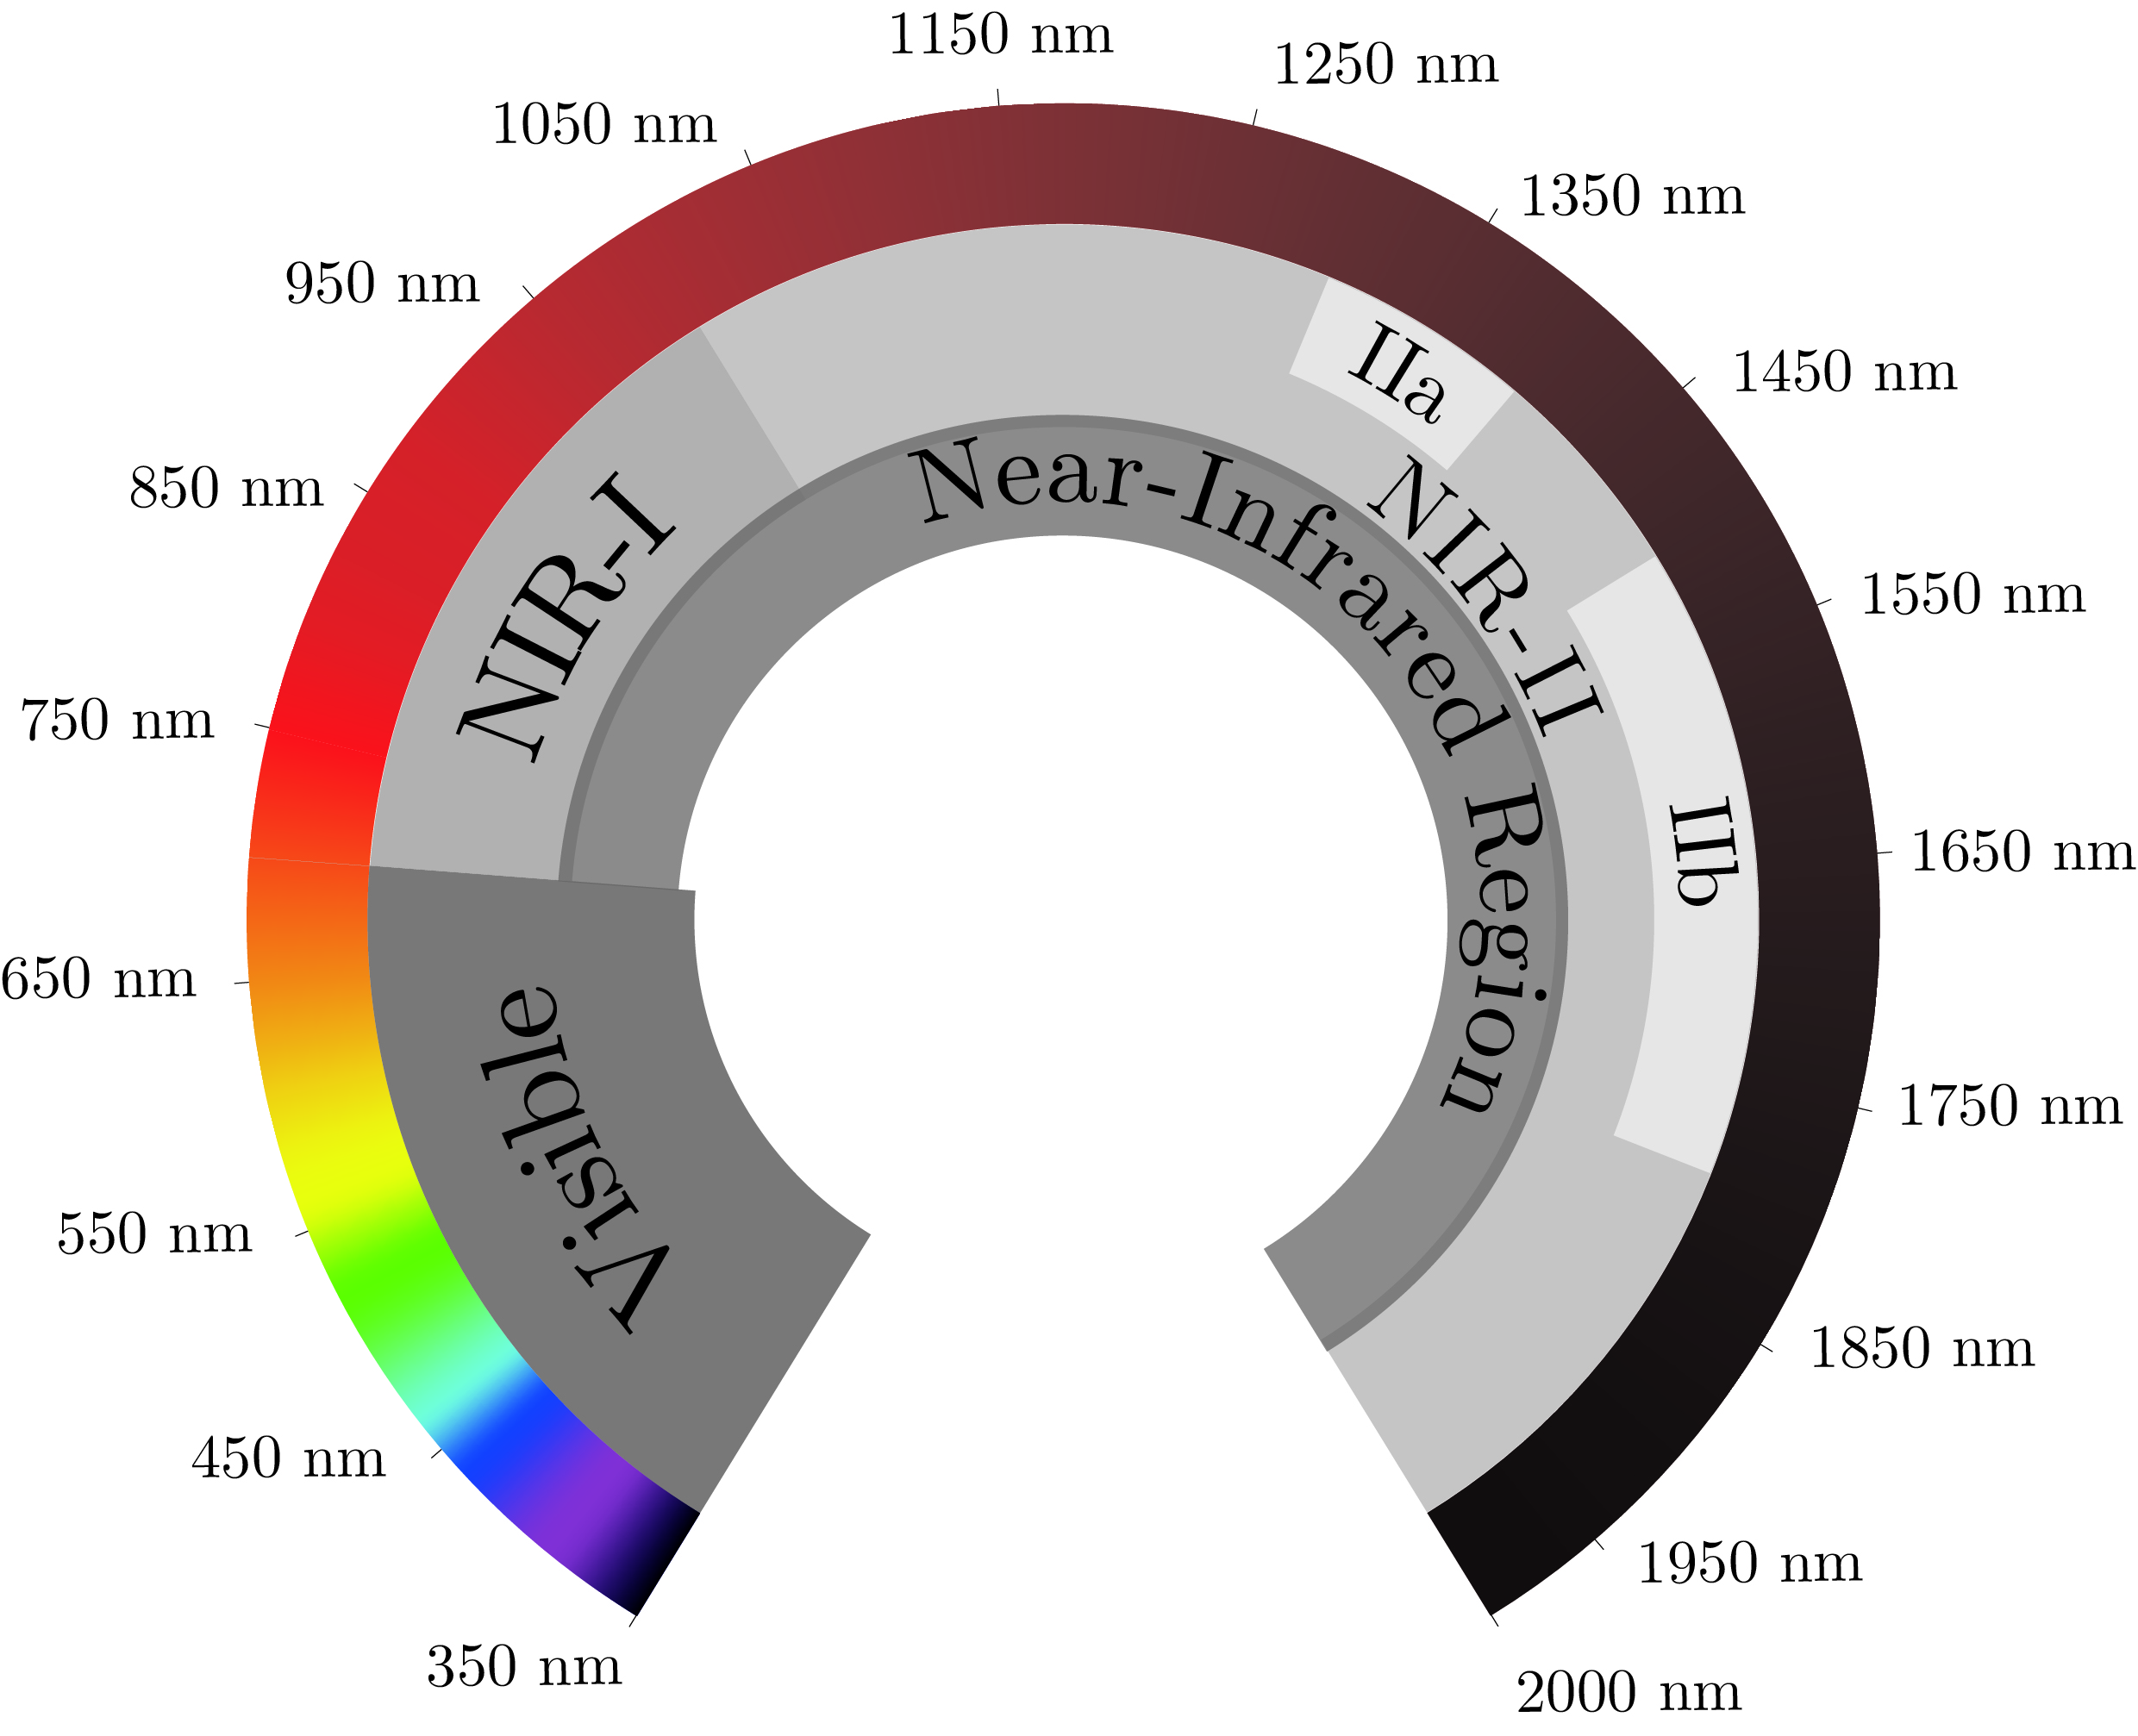
\includegraphics[width=0.8\textwidth]{near_infrared_theory/EMspectrum_VISNIR}
%
% If no graphics program available, insert a blank space i.e. use
%\picplace{5cm}{2cm} % Give the correct figure height and width in cm
%
\caption{Spectrum of visible and near infrared light with the most common imaging subwindows.}
\label{fig:theory_em_spectrum}       % Give a unique label
\end{figure}

\subsection{Basic Interactions Between Light and Matter}
The propagation of light through tissues is a very complex phenomenon and is still a subject under study nowadays. The two main interactions that characterize it are absorption and scattering. Before going in depth into their physical meaning, it is very important to understand that energy exchanges with the medium occur within an energetic balance, having fundamental laws that must be preserved.

The fact that light is of electromagnetic nature ties it to one of the most elementary theorems in physics: energy conservation. Whatever happens during propagation, energy must be preserved. This property is the starting point to derive the equations that describe the flux of light through tissues.

The general equation of the theorem of energy conservation derived from the Poynting's theorem has the expression:

\begin{equation}
\frac{\partial W}{\partial t}+\frac{dP_{abs}}{dV}+\nabla \cdot S=0
\label{eq:theory_Ptheorem}
\end{equation}
The first term in (\ref{eq:theory_Ptheorem}) describes the variation of energy density with time, the second the absorbed power and the third the energy exchange with the medium due to incoming and outgoing energy. 

The Poynting's vector describes the energy flow of an electromagnetic wave as the cross product of the electric and the magnetic fields and is directly related to what we can actually measure with the instrumentation.

This expression must always hold in the far-field\textemdash distances of several wavelengths\textemdash and, in the case of light, the particularization in terms of the statistical approximation of the optical properties of the medium will lead to the \gls{rte}, which is the main equation for energy transport that accounts for scattering, absorption and emission in a statistical manner. The detailed derivation of the RTE is out of the scope of this chapter, however, we will try to give a general idea of the meaning behind it.

Keeping in mind the theorem of energy conservation (\ref{eq:theory_Ptheorem}), we will start now describing the main interactions that occur in tissues: absorption and scattering.

From a macroscopic point of view, absorption can be described as the energy dissipation that is produced during the interaction of an electromagnetic wave with matter. However, this process is rather more complex if studied from a particle point of view.

At room temperature, by default electrons from a particle, be it an atom or a molecule, can be found in a ground energetic state. Here we must point out that in the ground state (see Fig. \ref{fig:theory_jablonsky}, where it is defined as singlet state $\text{S}_0$), its electronic configuration is in the lowest available energy state given the conditions of the environment. When the incident light reaches the particle, the molecule or atom will be taken to an excited state, as long as the incident energy is enough to reach it. This means that electrons will be promoted to higher energy orbitals. Now, the molecule will tend to return back into the ground state by releasing the absorbed energy. This relaxation can occur in several ways, giving different results depending on the transition path and the excited state reached after the process.

The levels and sublevels of excitation that a particle can reach depend on the relative orientation of electron spins and the nature of the orbitals. These levels can be of two types: singlet $\text{S}_1$, $\text{S}_2$ and triplet $\text{T}_1$ state. Singlet states mean that all spins are paired\textemdash up/down\textemdash and have a multiplicity of $\text{M}=2\text{S}+1=1$. A triplet state, on the other hand, has two spins in the same state, thus reaching a multiplicity of $2\text{S}+1=3$. The most common situation is that the particle reaches a singlet state. In this case, during de-excitation, the energy can be liberated following two energetic paths. Energy can be delivered into the system in form of heat due to vibrational relaxation or it can be released through fluorescence emission. In the latter, the emitted electromagnetic radiation will be of lower energy\textemdash longer wavelength\textemdash since some energy is lost in the process. 

\begin{figure}[]
\centering
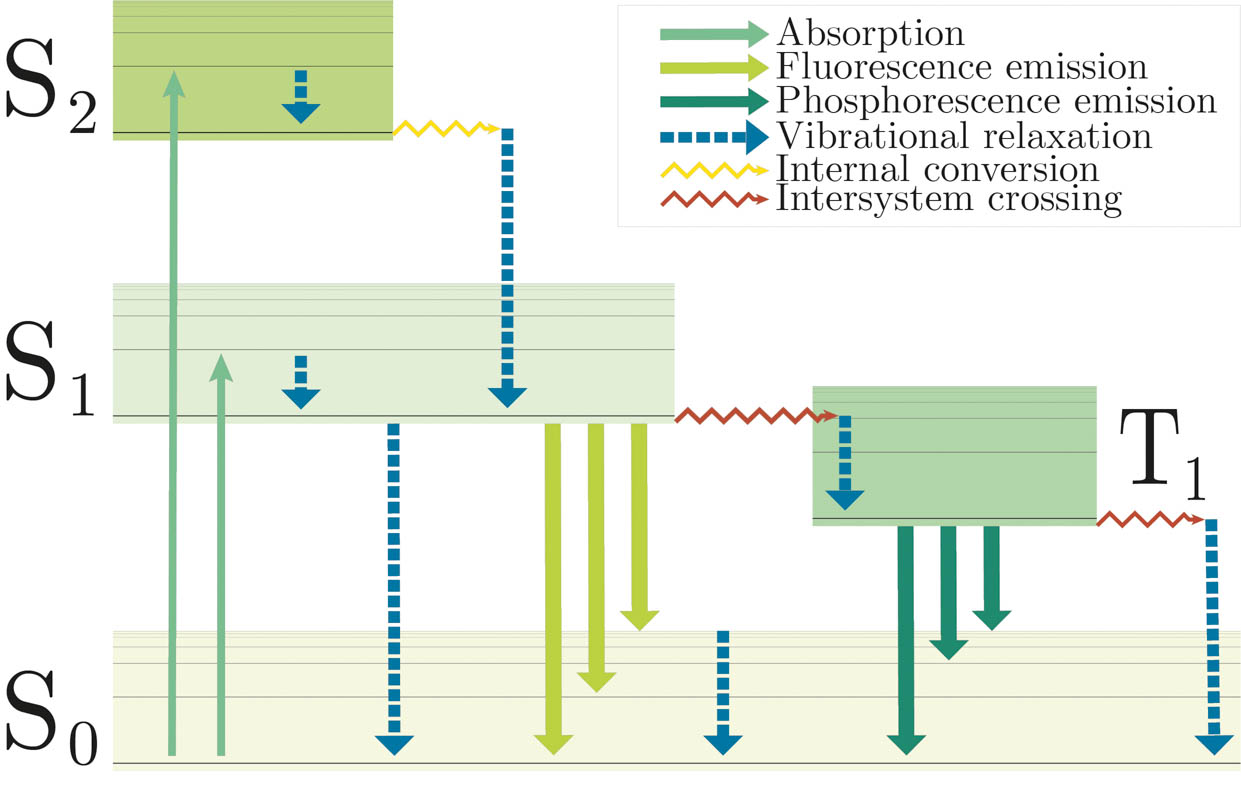
\includegraphics[width=0.8\textwidth]{near_infrared_theory/Jablonsky}
\caption{Perrin-Jablonsky diagram of the de-excitation pathways of a particle.}
\label{fig:theory_jablonsky}       
\end{figure}

Alternatively, during de-excitation the particle can turn into a triplet state through intersystem crossing. Since it is a lower energy state, the particle can then easily relax to the ground state either through internal conversion or through what we call phosphorescence which has very long lifetimes, due to the fact that a triplet-singlet ($\text{T}_1\rightarrow \text{S}_0$) transition is in principle forbidden due to Hund's rule. 

It is important to point out that processes of fluorescence have lifetimes in the order of tens to hundreds of nanoseconds. However, phosphorescence can be a much slower process, having a delay that can go from fractions of a second up to a few seconds, minutes, or even hours. All these processes and paths of excitation and de-excitation are depicted in Jablonsky diagrams as in Figure~\ref{fig:theory_jablonsky}.

Absorption accounts for the radiation that is dissipated without re-emission of light. For a single particle, it can be estimated by measuring the amount of power loss due to its interaction with an incident electromagnetic wave. The ratio of incident energy $\vert\langle \mathbf{S}^{(inc)}\rangle\vert$ in [\si{\W}]
and absorbed power $\overline{P_{abs}}$ in [\si{\W\per\cm\squared}] defines the absorption cross section $\sigma_a$:

\begin{flalign}
&&\sigma_a &=\frac{\overline{P_{abs}}}{\vert\langle\mathbf{S}^{(inc)}\rangle\vert},
\unit{\si{\cm\squared}}
%&&\left[\text{\si{\cm\squared}}\right]
%\tagaddtext{\left[\si{\cm\squared}\right]}
\label{eq:theory_sigma_a}
\end{flalign}

The absorption-cross section of a particle represents the effective cross section compared to its geometrical cross section in area units. This value represents only the absorption for a single particle, while, in bioimaging, it is much more useful to calculate the equivalent for a statistical ensemble of $N$ particles per unit volume $V$, represented by the absorption coefficient \gls{mua}:

\begin{flalign}
&& \mu_a & =\rho\sigma_a,
%&& \left[\text{\si{\per\cm}}\right]\quad
\unit{\si[per-mode=reciprocal]{\per\cm}}
\label{eq:theory_mu_a}
\shortintertext{where} 
&& \rho  &=\frac{N}{V},
\unit{\si{\particles\per\cubic\cm}}
%&& \left[\text{particles \si{\per\cm\cubed}}\right]
\end{flalign}

Absorption is the main limiting property in terms of how deep light can penetrate in tissues, since it removes energy of the incident wavelength as light propagates within the medium. Absorption attenuates the incident light, converting it into either vibrations of the medium\textemdash heat\textemdash through non-radiative processes, or emission of light of different wavelengths through radiative processes (fluorescence, phosphorence, and in specific cases of shorter wavelengths of emission, upconversion).

The re-emission of the incident radiation is known as scattering and practical cases of light propagation theory with in-vivo applications, only light re-emitted with the same frequency is considered. In this case, the phenomenon is specifically termed elastic scattering. In addition to the arrangement of the particles, the amount of scattering of a medium depends also on the size, shape and spatial distribution of these scatterers.

In Mie theory \cite{Mie1908}, the probability for an incident wave of being scattered into a certain direction depends on the relative size of the particle with respect to the incident wavelength. When particles in the medium are smaller, light is scattered as an outgoing spherical wave. This solution to the Mie theory is known as Rayleigh scattering. When there is a slight index of refraction mismatch, such as between cells and the surrounding extracellular medium, as the size of the particle increases the scattered radiation deviates from that of an outgoing spherical wave, peaking in the forward scattering direction.

The scattering cross-section $\sigma_s$ quantifies the scattering efficiency of a particle. This can be obtained by calculating the ratio between the scattered power $\overline{P_{sc}}$ and the incident energy. However, given the directional dependence of scattering, it can be also estimated as the integral of the scattering amplitude $\vert f\left(\mathbf{\hat{s}},\mathbf{\hat{s}}_0\right)\vert$ over all angles. The scattering amplitude accounts for the contribution of the scattered wave to a certain direction $\mathbf{\hat{s}}$, given an incident direction $\mathbf{\hat{s}}_0$. Hence, the scattering cross-section gives information about the probability of light of being scattered, no matter the direction, and is defined as:

\begin{flalign}
&&\sigma_s &=\frac{\overline{P_{sc}}}{\vert\langle \mathbf{S}^{(inc)}\lvert\rangle\rvert}=\int_{\left(4\pi\right)}\left| f\left(\mathbf{\hat{s}},\mathbf{\hat{s}}_0\right)\right|^2d\Omega,
\unit{\si{\cm\squared}}
%\qquad\left(\text{cm}^2\right)
\label{eq:theory_sigma_s}
\end{flalign}

The scattering coefficient \gls{mus} can be estimated similarly to the absorption coefficient for a known density of particles in the medium.

\begin{flalign}
&&\mu_{s}&=\rho\sigma_s,
\unit{\si[per-mode=reciprocal]{\per\cm}}
\label{eq:theory_mu_s}
\end{flalign}

In biological tissues, cells can be considered as the main scatterers. As they are quite transparent and their average size is usually greater than the wavelengths used for imaging, the angular distribution of the scattered light becomes highly anisotropic mainly due to the small index of refraction mismatch between different tissue components. Therefore, the description of scattering in tissues must account for this effect. The anisotropy factor \gls{g} represents the average cosine of the angle between the incident wave and the scattered. This unitless parameter takes values from $-1$ to $1$, being $-1$ fully backward scattering and $1$ only forward. A particle with perfect isotropic scattering would have a value of $0$. In terms of scattering, and neglecting absorption, this coefficient informs about how much transparent is the medium. 

The anisotropy factor is included in the model through the reduced scattering coefficient, with the expression:
\begin{flalign}
&&\mu'_s &=\left(1-g\right)\mu_s
\unit{\si[per-mode=reciprocal]{\per\cm}}
\label{eq:theory_mu_s_prime}
\end{flalign}

As an example, a highly scattering medium with a scattering coefficient of \SI[per-mode=reciprocal]{110}{\per\cm} can decrease its effective scattering through the reduced scattering coefficient if its anisotropy is $0.9$ to \SI[per-mode=reciprocal]{1.10}{\per\cm}. Usually, biological tissues have very high scattering anisotropy, taking values that range from $g=0.8$ to $g=0.9$~\cite{Jacques2013}.

The scattering coefficient follows a negative power law with respect to the wavelength, thus decreasing as wavelength increases. This dependence is monotonic, due to the small size of the particles with respect to the wavelengths considered.

The dependence of the angular distribution of scattering on the relative size between the wavelength and the particle's makes the scattering coefficient value to follow a negative power law with respect to the wavelength, thus for tissues decreases as wavelength increases with monotonic dependence.

It is important to remark that the statistical definition of the optical properties in terms of their relative cross-sections and particle densities is valid for biological tissues only because the variations on the properties within the medium are assumed to be very smooth. Also, the constant movement of cells (motility) induces a self-averaging effect to the local light intensity. This property cancels any effect coming from constructive or destructive interference in the case of using coherent illumination.

Before moving into the physics of light propagation, two more important coefficients must be defined using the quantities of scattering, absorption and anisotropy. The transport coefficient \gls{mutrr} accounts for scattering and absorption together. This important parameter is especially relevant when modeling propagation using Beer-Lambert's law (in absence or negligible scattering) as will be seen in following sections.

\begin{flalign}
&&\mu'_{tr}&=\mu'_s+\mu_a=\left(1-g\right)\mu_s+\mu_a,
\unit{\si[per-mode=reciprocal]{\per\cm}}
\label{eq:theory_mu_tr}
\end{flalign}

A direct consequence of the definition of the transport coefficient is the Transport Mean Free Path (tmfp, \gls{ltr}), also called Transport Length. This parameter is key to determine the degree of diffusiveness of light because it represents the mean distance that light must travel in the medium in order to become totally isotropic in propagation and hence loose its original directionality. This term is defined as the inverse of the transport coefficient:

\begin{flalign}
&&l^*_{tr}&=\frac{1}{\mu'_{tr}}=\frac{1}{\mu'_s+\mu_a},
\unit{\si{cm}}
\label{eq:theory_l_tr}
\end{flalign}

\section{Light Propagation in Biological Tissues}
Once the optical properties of tissues have been defined, we will try to understand how light propagates through tissues. In turbid media, propagation is modeled by the diffusion approximation of the diffusion equation. The derivation of this expression is beyond the purposes of this chapter, and therefore, we will only give an overview of the steps to reach it, explaining the purpose of each of them.

The path towards deriving the diffusion equation from radiative transfer theory~\cite{Ishimaru1978} begins by recovering the equation of energy conservation and rewriting it to include the absorption and scattering coefficients that we described in the previous section. For that, the energy must be expressed in terms of the specific intensity \gls{I}, [\si[per-mode=reciprocal]{\watt\per\centi\metre\squared\per\steradian}]. This quantity represents the average flow of energy at a point $\mathbf{r}$ in a certain direction $\mathbf{\hat{s}}$. It is calculated through the integration of the discrete interaction of every incident wave\textemdash Poynting vector\textemdash with the scatterers and absorbers within a small volume. This is equivalent to estimating the average Poynting vector within this small volume in a certain direction.

When the equation for energy conservation is expressed in terms of the specific intensity, we obtain the RTE, which models the energy flow in a medium through the evaluation of its intensity in a certain direction in small volumes with homogeneous optical properties. The expression for a system where a certain amount of energy $\epsilon(\mathbf{r},\mathbf{\hat{s}})$ [\si[per-mode=reciprocal]{\watt\per\second\per\cm\cubed}] is introduced by a source is represented by the RTE: 
\begin{equation}
\frac{1}{c_0}\frac{\partial}{\partial t}I(\mathbf{r},\mathbf{\hat{s}})+
\mathbf{\hat{s}}\cdot\nabla I(\mathbf{r},\mathbf{\hat{s}})+
\mu_tI(\mathbf{r},\mathbf{\hat{s}})-\mu_t\int_{(4\pi)}I(\mathbf{r},\mathbf{\hat{s}'})p(\mathbf{\hat{s}},\mathbf{\hat{s}}')d\Omega'=
\epsilon(\mathbf{r},\mathbf{\hat{s}})
\label{eq:theory_rte}
\end{equation}

Then, if the directional information is integrated, an equivalent expression to the RTE will be reached (\ref{eq:theory_rte_en_cons}), however this time in terms of the average intensity \gls{Ur} and the flux \gls{Jr} for each position. Here, it is important to remember that the average energy for every point is calculated using the average intensity within small volumes of the medium. This time, the result of the integral over the energy introduced into the system is the source term $S_o\left(\mathbf{r}\right)$ [\si[per-mode=reciprocal]{\watt\per\centi\metre\cubed}].
\begin{equation}
\frac{1}{c_0}\frac{\partial}{\partial t}U(\mathbf{r})+
\nabla\cdot\mathbf{J}(\mathbf{r})+
\mu_tU(\mathbf{r})-
\mu_sU(\mathbf{r})=
S_0(\mathbf{r})
\label{eq:theory_rte_en_cons}
\end{equation}

The terms in (\ref{eq:theory_rte_en_cons}) represent each of these quantities:

\begin{itemize}
\item The first term represents the variation of the average intensity at $\mathbf{r}$ with time. 
\item The second term describes the energy flux coming and leaving the volume.
\item The next term accounts for the losses due to absorption and scattering. The latter here refers to the amount of energy that is scattered out of the volume considered at \textbf{r} and hence is accounted as loses.
\item The last term is also referred to scattering, but in this case is describing the energy that is coming into the volume scattered by the areas surrounding. Therefore, this term has a negative sign in the equation.
\end{itemize}

The RTE can model nearly any situation regarding light propagation. Before particularizing it for diffusion, it is interesting to analyze the case in which the contributions from scattering can be neglected. Here, the medium would have a very small scattering coefficient, and hence the term that accounts for contributions from adjacent volumes can be eliminated from the expression. Assuming also no external sources and constant illumination, the equation would become:

\begin{equation}
\nabla\cdot\mathbf{J}\left(\mathbf{r}\right)+\mu_t U\left(\mathbf{r}\right)=0
\label{eq:theory_beer_law}
\end{equation}

This expression represents the modified \gls{bl} Law for light propagation. Here, the variation of the flux of energy\textemdash which represents the fluctuation of energy density in a volume\textemdash is only caused by attenuation of the average intensity in terms of the transport coefficient (see Fig.~\ref{fig:theory_beer}). The solution to this expression is simply an exponentially decaying intensity without any spatial change in the spatial distribution of the intensity in propagation.

\begin{figure}[]
\sidecaption[t]
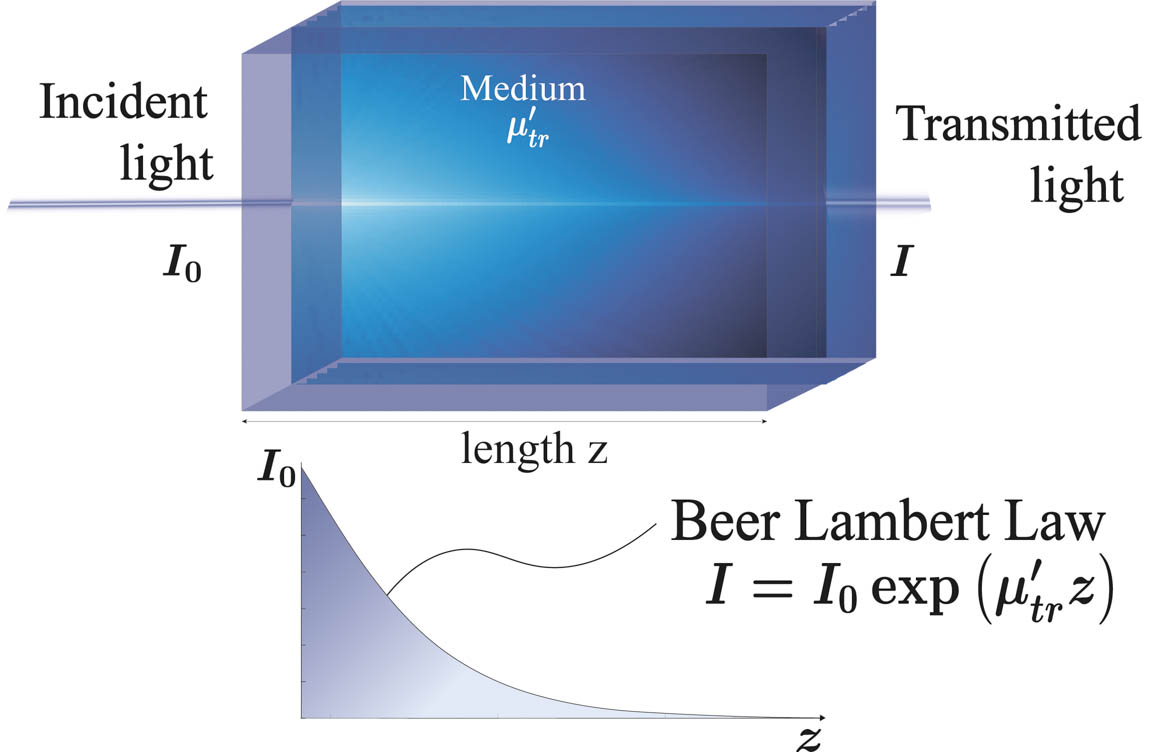
\includegraphics[width=0.65\textwidth]{near_infrared_theory/Beer_slab_v}
\caption[Illustration of the Beer-Lambert Law]{Illustration of the Beer-Lambert law. Light transmitted in a scattering free medium has an exponentially decaying intensity without any variation in its spatial distribution along the propagation axis.}
\label{fig:theory_beer} 
\end{figure}

The diffusion approximation aims to simplify the RTE by adding some conditions and assumptions that will help to reach an analytic solution. Through these approximations, we will obtain an expression for the average intensity \gls{Ur} that represents the light distribution in diffusive media. Here, we will mention the most important ones, explaining their limitations and consequences in the solution of the light propagation equation.

The diffusion equation is based on Fick's law. These establish that the flux of energy flows from high concentration regions to others with lower concentration, creating a gradient of energy that depends on a constant termed the diffusion coefficient ($D$). This parameter is usually expressed in terms of the properties of the medium and regulates the amount of energy flow. The expression for the flux \gls{Jr} in terms of the gradient of the average intensity becomes:
\begin{equation}
\mathbf{J}\left(\mathbf{r},t\right)=-D\nabla U\left(\mathbf{r},t\right)
\label{eq:theory_fick}
\end{equation}

Before introducing the main approximation that will help to find an expression for the specific intensity, it is important to point out that in diffusion theory, light intensity flowing in the medium is divided into two components \cite{Ishimaru1978}:

\begin{itemize}
\item \textit{Reduced intensity}, \gls{Iri}: ballistic contribution of light that still has high directionality.
\item \textit{Diffuse intensity} \gls{Id}: corresponds to light that has already being scattered several times and therefore has lost its initial directionality and whose flux follows Fick's law (see \ref{eq:theory_fick}).
\end{itemize}

At the vicinity of the source, most of the contribution to the intensity will be from the reduced component. However, after several scattering events, it will loose completely its original direction of propagation, being its energy gradually transferred to the diffuse intensity. At a point \textbf{r} in the medium, the intensity will be a combination of these two components. Equivalently, this step has attached the definition of the corresponding average reduced and diffuse intensities, \gls{Uri} and \gls{Jri}, and fluxes \gls{Jri} and \gls{Udr}. 

In order to reach the solution of the diffusion problem, an estimation for the diffuse intensity must be introduced (since the reduced is given by the source, following Beer-Lambert's law). The definition of the angular distribution of the specific intensity is the main approximation within the diffusion approximation. It assumes that the diffuse component of the intensity can be modeled as the combination of the contributions of a uniform average intensity and a flux pointing in a certain direction (see Fig.~\ref{fig:theory_ang_dist}). Mathematically, it corresponds to a first order spherical harmonic expansion, leading to the following expression:
\begin{equation}
I_d\left(\mathbf{r},\mathbf{\hat{s}}\right)=
\frac{U_d\left(\mathbf{r}\right)}{4\pi}+
\frac{3}{4\pi}\mathbf{J}_d(\mathbf{r})\cdot\mathbf{\hat{s}}
\label{eq:theory_ang_dist}
\end{equation}

\begin{figure}[]
\sidecaption[]
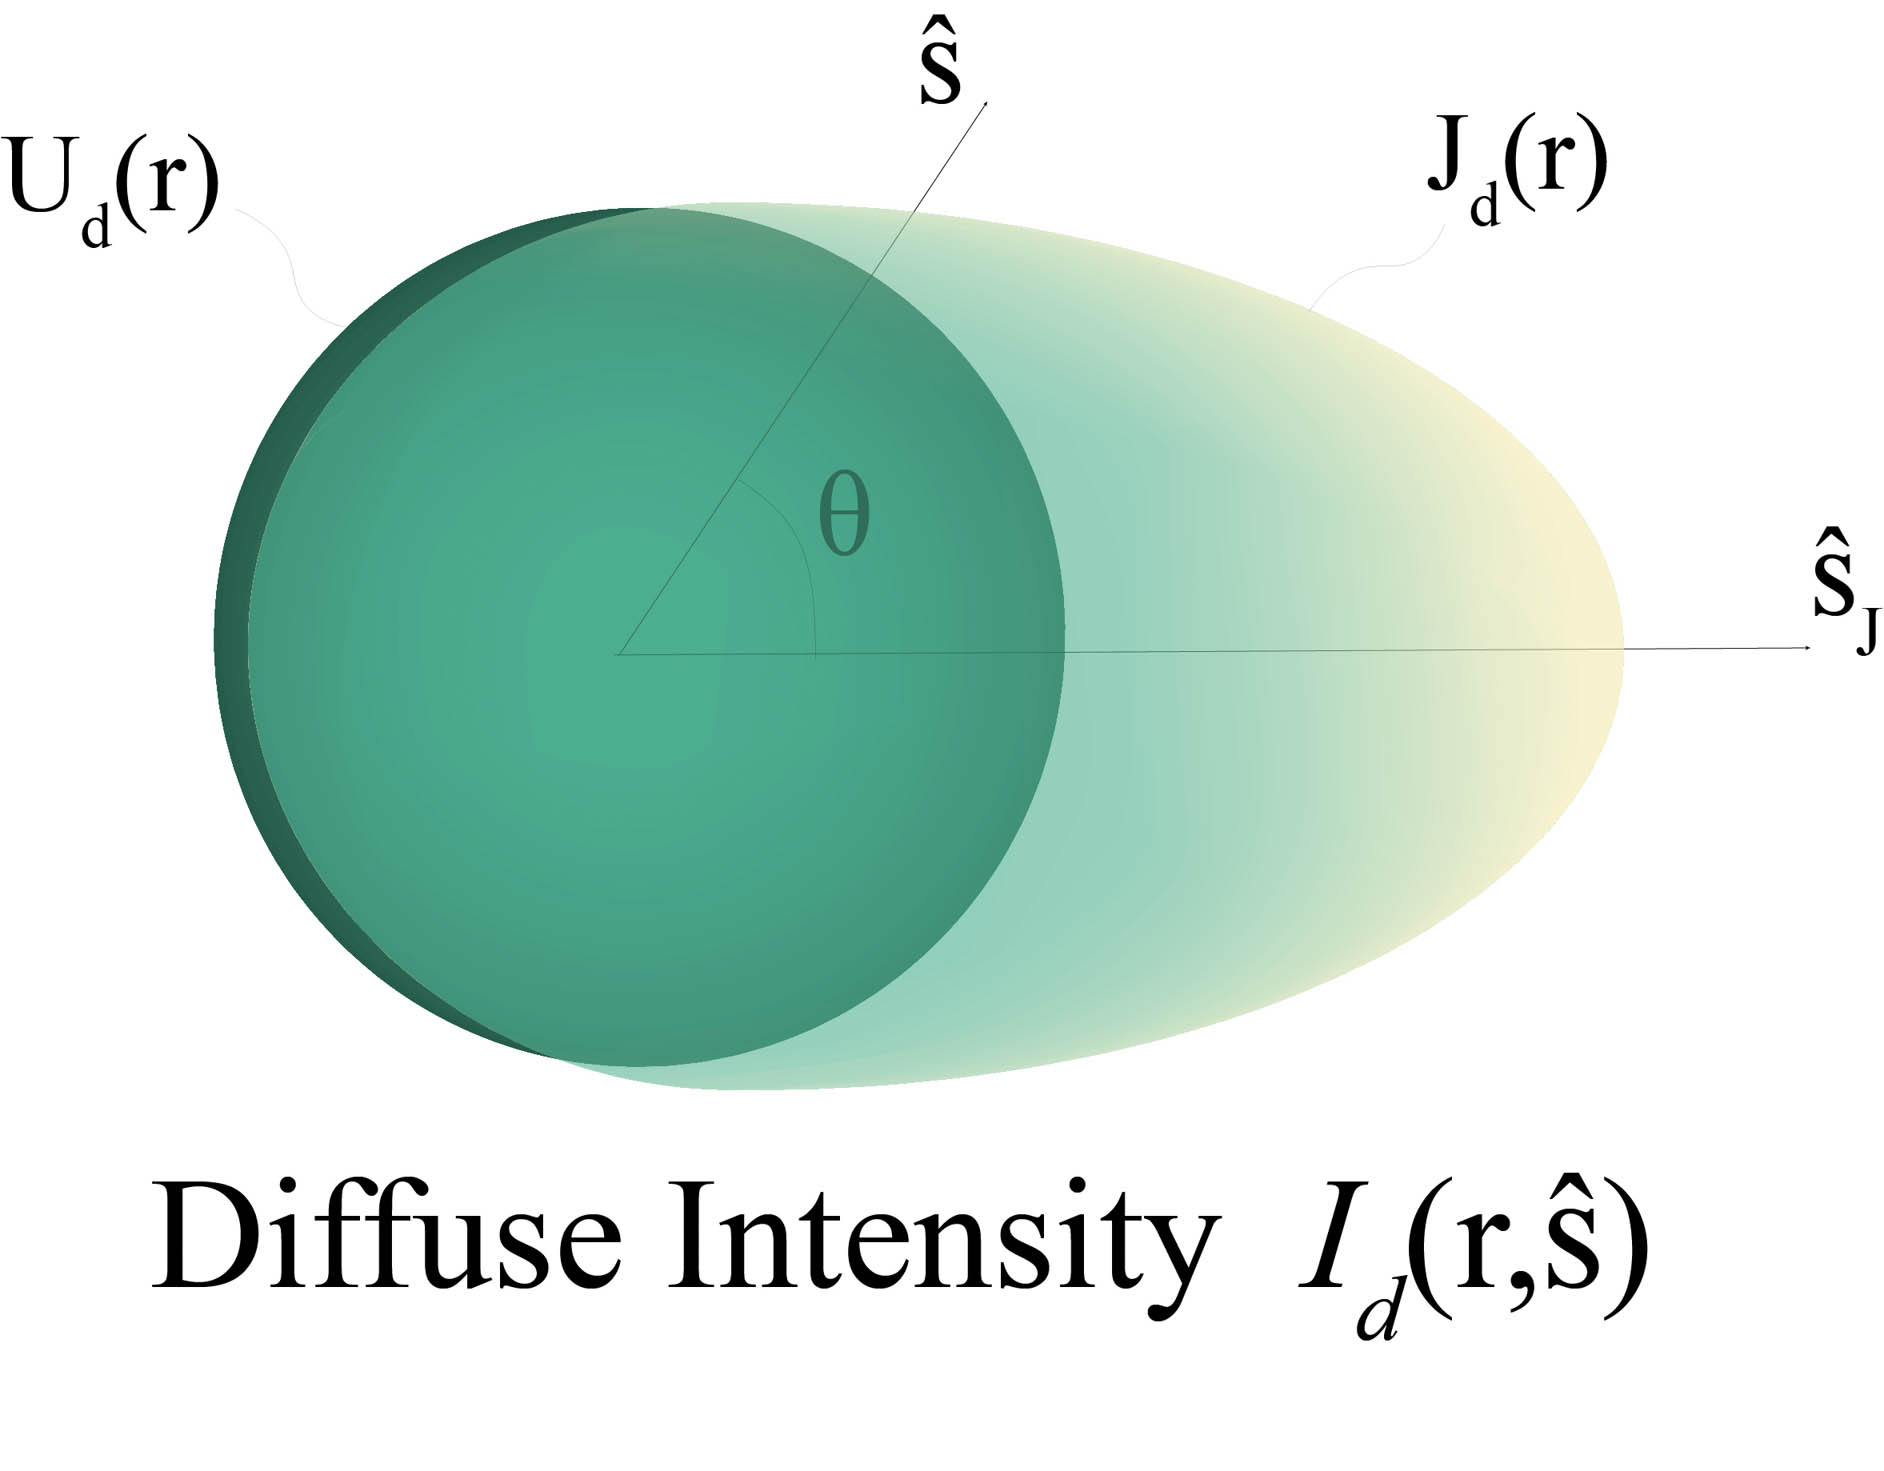
\includegraphics[width=0.6\textwidth]{near_infrared_theory/angular_distribution}
\caption[Angular distribution of diffuse light.]{Approximation of the diffuse intensity as a first order spherical harmonic. The illustration depicts the angular dependence of the diffuse intensity.}
\label{fig:theory_ang_dist} 
\end{figure}

This approximation incorporates essential information from the distribution of the diffuse specific intensity and allows to find an expression for the diffusion coefficient. If the definition for the diffuse intensity is introduced into the RTE and then again integrating over all angles to obtain the expression for the flux $\mathbf{J}_d$ can be found:
\begin{equation}
\mathbf{J}_d=-\frac{1}{3\left(\mu'_s+\mu_a\right)}\nabla U_d\left(\mathbf{r},t\right)
\label{eq:theory_dif_flux}
\end{equation}
This expression is Fick's law from which the diffusion coefficient \gls{D} can be easily extracted:
\begin{flalign}
&& D &=\frac{1}{3\left(\mu'_s+\mu_a\right)}
\unit{\si{\cm}}
\label{eq:theory_dif_coeff}
\end{flalign}

The last step to finally reach the diffusion approximation is to introduce the expression for the diffuse flux into the equation for energy conservation (\ref{eq:theory_rte_en_cons}), which yields:
\begin{equation}
\frac{1}{c_0}\frac{\partial}{\partial t}U_d\left(\mathbf{r},t\right)+
\mu_aU_d\left(\mathbf{r},t\right)-
D\nabla^2U_d\left(\mathbf{r},t\right)=
\mu'_sU_{ri}\left(\mathbf{r},t\right)
\label{eq:theory_diff_aprx}
\end{equation}

In this equation, the only contribution to the reduced intensity, the ballistic component of light, comes from the source.
It is very interesting to notice that if constant illumination is assumed\textemdash no temporal variation\textemdash the diffusion equation can be rewritten as a Helmholtz equation, using the relationship:
\begin{equation}
k_0^2=-\frac{\mu_a}{D}
\label{eq:theory_k_0}
\end{equation}

The expression now becomes:
\begin{equation}
\left(\nabla^2+k_0^2\right)U\left(\mathbf{r}\right)=-\frac{\mu'_s}{D}U_{ri}\left(\mathbf{r},t\right)
\label{eq:theory_helmholtz}
\end{equation}

This change allows to transform it into an inhomogeneous differential equation whose solution for a point source is:
\begin{equation}
U(\mathbf{r})=S_0\frac{\text{exp}\left(ik_0\mathbf{r}\right)}{4\pi D\mathbf{r}}
\label{eq:theory_green}
\end{equation}

The expression above represents the intensity distribution of a point source propagating in a diffusive medium.

\section{Optical Properties of Tissues in the Near Infrared}
\label{sec:2}
The previous section presented a description of the physics that characterize the propagation of light in tissues. The optical properties are not constant along the spectrum, taking different values for scattering and absorption depending on the chromophores, particle sizes and shapes present in the tissues and the incident wavelength. 
In this section, we aim to describe the scattering and absorption spectra in the visible and NIR for the components of the tissues that have the greatest impact on imaging: blood, water and skin. The study of the behavior of light at different wavelengths will help to understand why NIR light is so advantageous for imaging and the considerations that must be taken when designing optical systems.

\subsection{Blood}

Blood is the main absorber in tissues due to the strong presence of hemoglobin, which is the vehicle for oxygen transport. This chromophore constitutes up to 97\% of red blood cells composition which conform approximately 50\% of the whole blood's volume. The other half are white cells, platelets and mainly plasma, which is nearly transparent due to its elevated content of water.
There are some differences between the absorption efficacy of oxygenated and de-oxygenated blood, being the first redder and therefore slightly more absorbent in the region within 600 and \SI{700}{\nm}. These properties enable several measurements of biomedical parameters such as blood oxygen saturation just by playing with the intensities that pass through a finger at different wavelengths.

In the NIR, both oxygenated and deoxygenated blood have a minimum in their absorption curve (see Fig. \ref{fig:theory_blood_spectrum}), becoming nearly two orders of magnitude more transparent than in the visible regime. Since blood is one of the main absorbers in the body, and given its strong presence in tissues, light in the NIR can penetrate much deeper than in the visible range. Moreover, the scattering coefficient decreases monotonically for longer wavelengths, increasing notably the transport mean free path of light in the NIR~\cite{Bosschaart2014}.

\begin{figure}
\centering
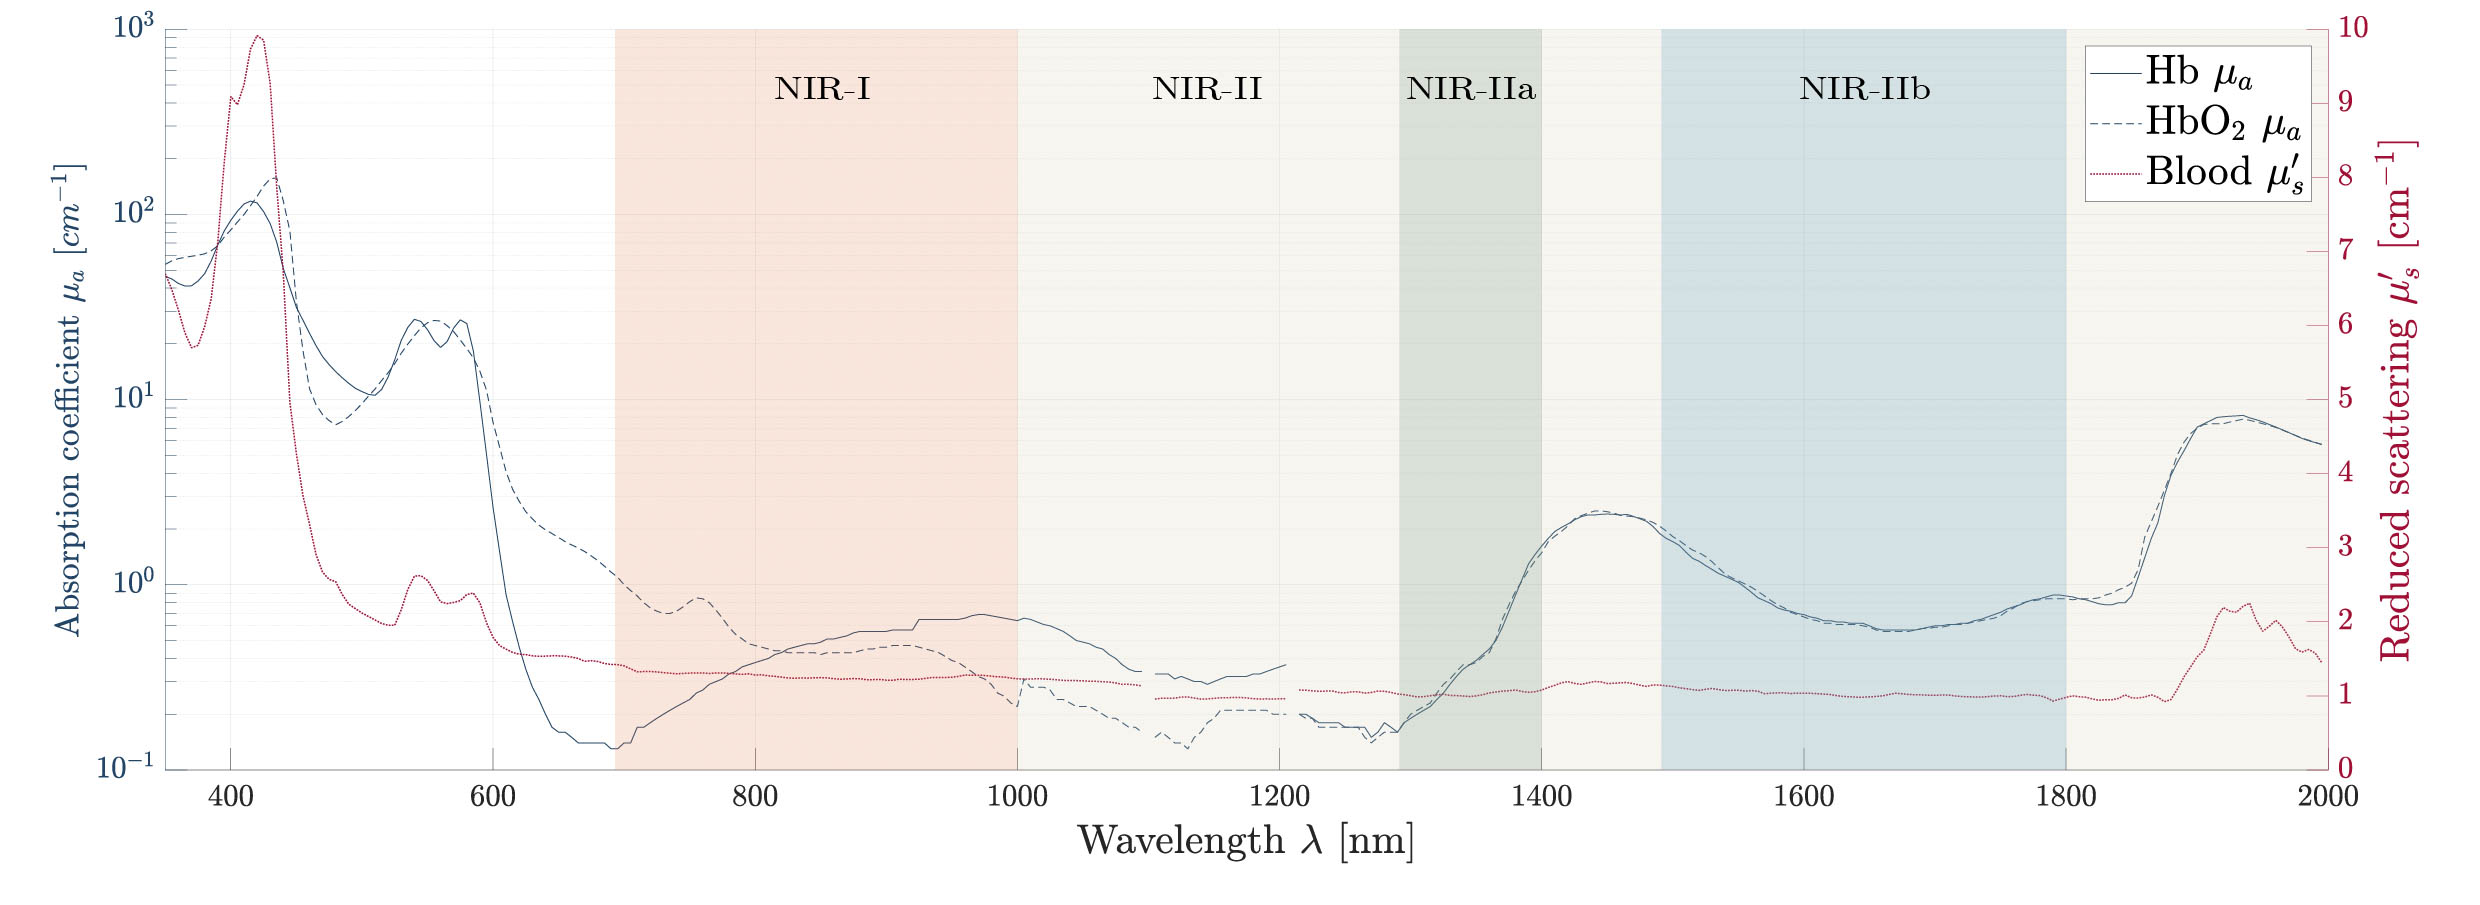
\includegraphics[width=\textwidth]{near_infrared_theory/blood_NIR}
\caption[Absorption and scattering spectra of blood]{Spectra of absorption and scattering of blood and water absorption. In the near infrared blood presents reduced scattering and less absorption compared to the visible region. Note that the absorption for oxygenated blood ($\mathrm{HbO_2}$) in the range from 600 to \SI{800}{\nm} is much lower than deoxygenated giving it its characteristic dark red color. Data interpolated from \cite{Bosschaart2014}.}
\label{fig:theory_blood_spectrum} 
\end{figure}


\subsection{Water}
Water absorption must be carefully taken into account for imaging since it is responsible\textemdash on average\textemdash of 60\% of human body weight. Its absorption spectrum reveals high transparency in the visible wavelengths, increasing significantly in the infrared. In fact, in the NIR, it can be up to 2 orders of magnitude more absorbent (see Fig.\ref{fig:theory_water_spectrum}). 

\begin{figure}[]
\centering
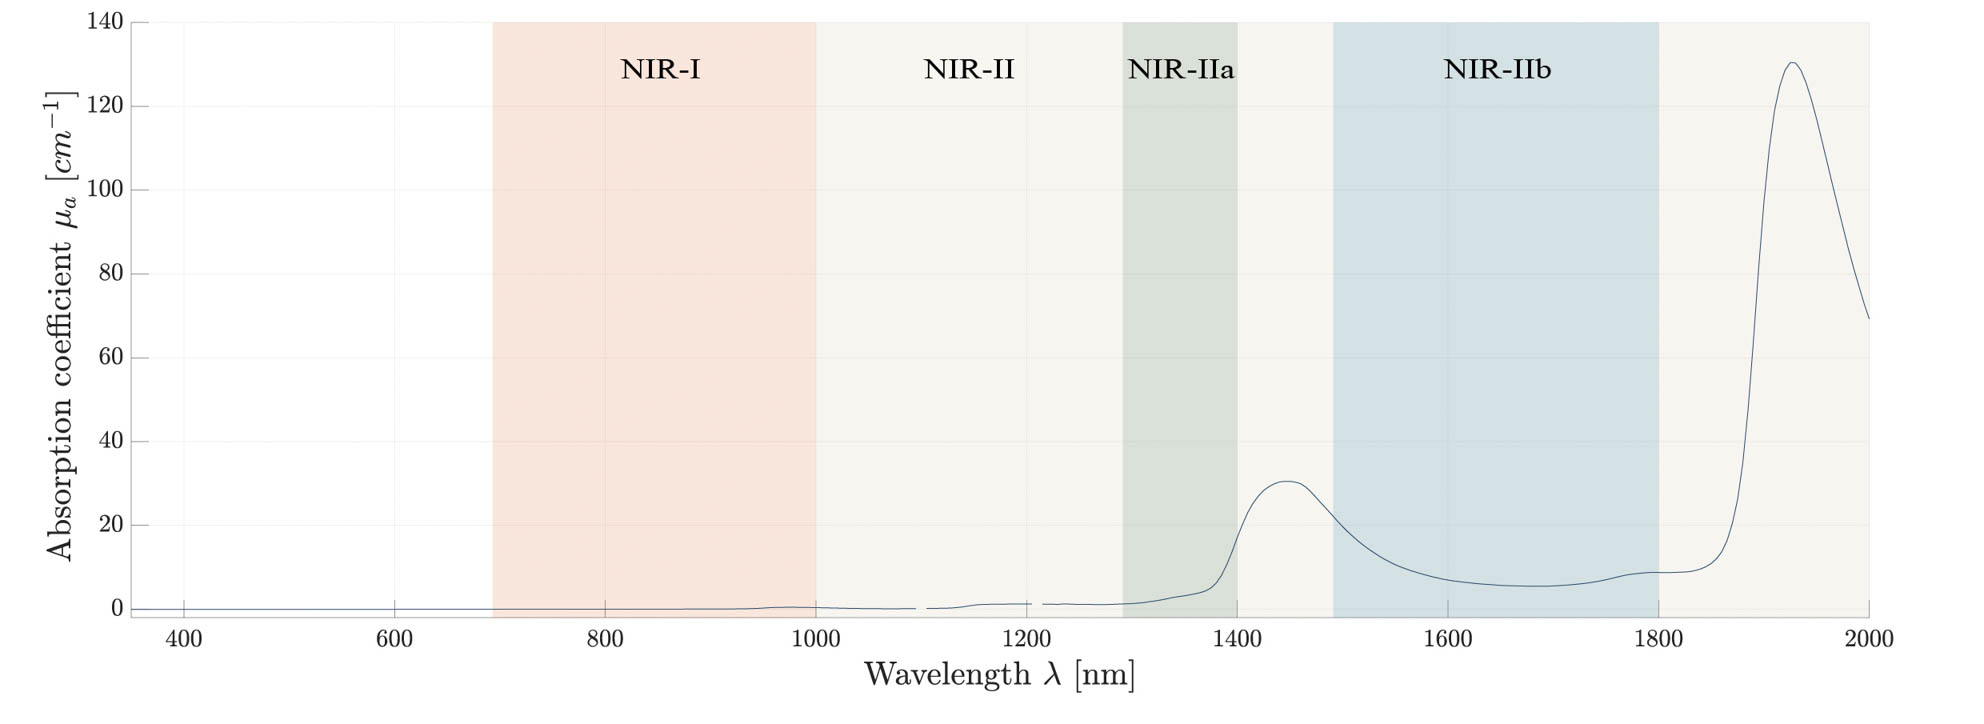
\includegraphics[width=1\textwidth]{near_infrared_theory/water_NIR}
\caption[Absorption spectrum of water.]{Absorption spectrum of water. Attenuation increases in the NIR region. The absorption peaks define the boundaries of the imaging windows. Data interpolated from Steve Jacques and Scott Prahl's website, \url{http://omlc.org/spectra}. }
\label{fig:theory_water_spectrum} 
\end{figure}

The water absorption coefficient curve has a sharp transition in the NIR, having a peak at \SI{1400}{\nm} that limits the penetration depth of light for this window. This maximum splits the \gls{nir2} window into the a and b regions. So far, during the design of the optimal working wavelength of an imaging system, this peak used to be avoided, using frequencies of the spectrum below or above. However, recent studies suggest that image contrast and penetration depth can be maximized at those wavelengths of greatest water absorption~\cite{Tanzid2016,Carr2018}.



\subsection{Skin}
Optical imaging techniques that aim to measure deep into tissues must traverse the skin. Its main chromophore is melanin, which is in charge of protecting the body against ultraviolet radiation by absorbing the harmful radiation and releasing it through vibrational relaxation as heat. Thus, skin absorption is very high between 300 and \SI{400}{\nm} (see Fig. \ref{fig:theory_melanin_spectrum}). 

The absorption coefficient of skin depends on the type and density of melanin that predominates, which gives a specific color depending on the subject. In general, experimental measurements of its optical properties reveal that at longer wavelengths than \SI{400}{\nm} absorption decreases, having a minimum region between the \gls{nir1} and \gls{nir2}a windows. In the \gls{nir2}b, the increase of absorbance of water slightly reduces the skin's transmittance. 
\begin{figure}
% \sidecaption[t]
\centering
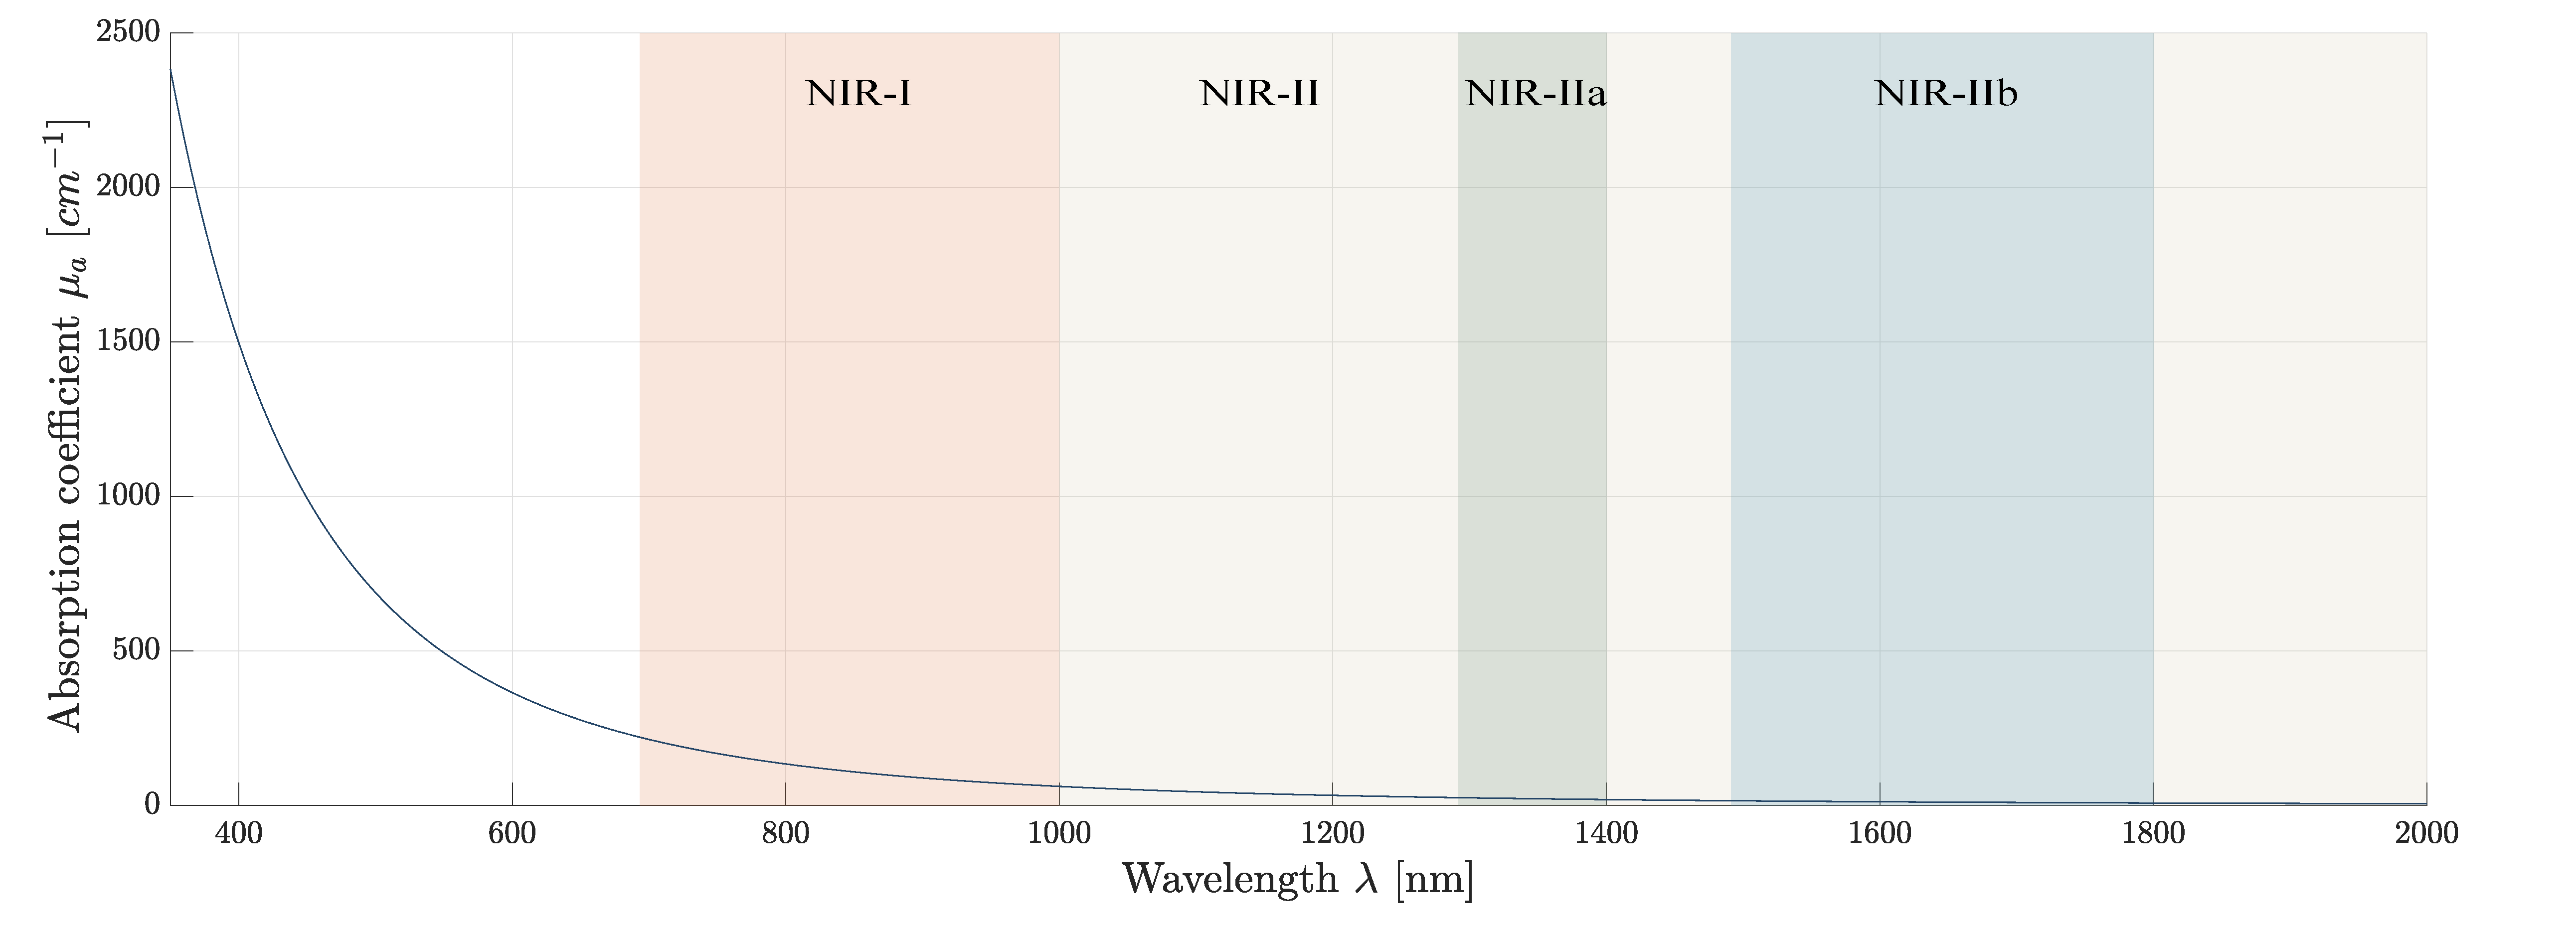
\includegraphics[width=1\textwidth]{near_infrared_theory/melanin_NIR}
\caption[Absorption spectrum of melanin.]{Absorption spectrum of melanin. Data generated using Steve Jacques and Scott Prahl's website, \url{http://omlc.org/spectra}. }
\label{fig:theory_melanin_spectrum} 
\end{figure}

In terms of depth of penetration, the best region to measure through skin is between 1000 and 1300 nm, however, as the scattering coefficient decreases for longer wavelengths, imaging in the II-b region is still favorable \cite{Bashkatov2005}.


\subsection{Tissue Autofluorescence}
Tissues by default have endogenous fluorescent components, each with different absorption and emission properties and lifetimes. In fluorescence imaging modalities, the excitation light can also activate these molecules, creating an ``endogenous'' background intensity in the images that decreases the signal to noise ratio, the sensitivity, and the fluorescent probe specificity.
This is especially critical for the cases where the fluorophore is located deep in the tissues and nearly no excitation illumination can reach it. In this scenario, increasing the exposure time of the sensor will also amplify the background intensity. 

Light in the NIR, especially in the \gls{nir2} window, presents two advantages that contribute to reduce the intensity from tissue autofluorescence. Firstly, the tissue autofluorescence is much lower than in the visible and \gls{nir1} windows. This is especially relevant for the \gls{nir2}a and \gls{nir2}b windows of the spectrum, where the autofluorescence intensity is almost negligible~\cite{Smith2009a}. Secondly, the increased depth of penetration and reduced scattering allows the excitation of the target fluorophore with more intensity and accuracy (due to lower scattering). In the \gls{nir1} window, a significant contribution to autofluorescence can still be found in melanin, inner organs and, in the specific case of mice, in the intestines mainly due to the presence of alfalfa~\cite{DelRosal2016}. This particular case may be significantly improved by switching to an alfalfa free diet. 



\section{Imaging in the II Near Infrared Window}
\label{sec:imaging}
As has been presented during the previous sections, imaging in the NIR has several advantages over the visible spectrum. Given the broad range of wavelengths it comprises, several NIR subwindows have been defined according to the optical properties of tissues. Recently, the latest detection instruments allowed imaging in the \gls{nir2} window, which has the most advantageous optical properties.

In general, most of the tissues with blood content present lower absorption and scattering rates in the \gls{nir2} window and in addition to the reduced autofluorescence, they contribute to an optimal scenario for fluorescence imaging. Techniques suffering from limited efficiency on the excitation of the fluorophore due to scattering such as \gls{lsfm}~\cite{Huisken2004, Olarte2018} can take advantage of NIR wavelengths to create planes of light that allow to scan through larger samples. Moreover, fluorophores with emissions in the \gls{nir2}a and \gls{nir2}b windows offer better possibilities in terms of contrast and resolution at depths up to several centimeters~\cite{Hong2014,Diao2015}. However, the number of fluorophores effective in this range is still very limited, specially those with tested biocompatibility~\cite{Hong2017}. Lately, some groups have started to explore the possibilities of traditional commercially available NIR dyes, such as the FDA-approved indocyanine green (ICG) for imaging in the \gls{nir2} window~\cite{Carr2018a}. Finally, other techniques such as \gls{opt}~\cite{Sharpe2002}, can notably improve their performance in terms of resolution and sample sizes using low scattering wavelengths~\cite{Fieramonti2012,Ripoll2009,Arranz2014}.

Although the optical properties in the \gls{nir2} region seem to be ideal, there is still much to do regarding the characterization of the propagation of light at these new imaging windows. The reduction in scattering increases the ballistic contribution of light (what was termed reduced intensity in (\ref{eq:theory_diff_aprx}), but the contribution of diffuse light still needs to be accounted for. Indeed, some approximations need to be revisited since the diffusion approximation on its own is not enough to properly model light propagation in this regime.

When propagating in very low scattering media, the contribution from the reduced intensity is higher than the expected by the diffusion equation \cite{Yoo1990}. This is the case of NIR light, where the transport length is much greater, hence measurements will be taken at distances where light has not become yet totally diffusive (or that still maintains some of its original directionality). When the transport mean free path increases, the transition from the ballistic to the diffusion regime takes place within up to several centimeters inside tissue (instead of millimeters as in the case of visible light), therefore the region with a high contribution of the reduced intensity is higher.

Under these conditions, one of the main approximations in the diffusion equation, the angular distribution of light based on a single angular component, might not be adequate. There are works using higher orders of spherical harmonic expansions to model the diffuse intensity, named the $P_n$ approximation \cite{Arridge2009}. Others try to find the distance in terms of the transport length where the transition from ballistic to diffusion propagation takes place \cite{Yaroshevsky2011}.

The study of the propagation of NIR light still has many unresolved issues. Currently the most common approach is to simulate the propagation using \gls{mc} methods\cite{WangJacquesZheng1995} and then try to refine the diffusion model \cite{Ripoll2005,Durduran1997,Spott2000} or the RTE \cite{tarvainen2005} to make them reproduce the results. Further investigations are needed to appropriately characterize the propagation in the NIR and improve the reconstruction methods. 

\section{Consequences of Near Infrared Light Propagation in Image Quality and Resolution}
\label{sec:resolution}
The previous sections of this chapter described the basics of light propagation in biomedical tissues. Additionally, the optical properties of tissues in the NIR and their consequences in diffusion theory were explained. This section aims to present from a practical point of view the consequences that the physics behind light propagation has when imaging in turbid media such as tissues. We will discuss the concept of resolution, how the properties of the medium affect it, and how light diffusion reduces image resolution as we image further from the objects studied.

The solution to the diffusion equation is an exponentially decaying outgoing spherical wave. Light emitted by an isotropic source, which could be a fluorescent bead, would propagate as displayed in Figure \ref{fig:theory_col_point_src}. The \gls{mc} simulation propagates light in a medium with low scattering, where diffusion is expected to hold at large distances from the source (approx. 1 cm, the inverse of the transport mean free path), only. If the source is collimated (see Fig.\ref{fig:theory_col_point_src}, bottom), as in the case of a laser beam, the effect of diffusion is much clearer from a visual point of view. Light has high directionality when entering the medium, but after traveling a very short distance, it loses it completely. Soon it starts propagating as a spherical wave centered inside the medium at a depth equivalent to one transport mean free path, as described by the solution of the diffusion equation.

\begin{figure}[t]
\centering
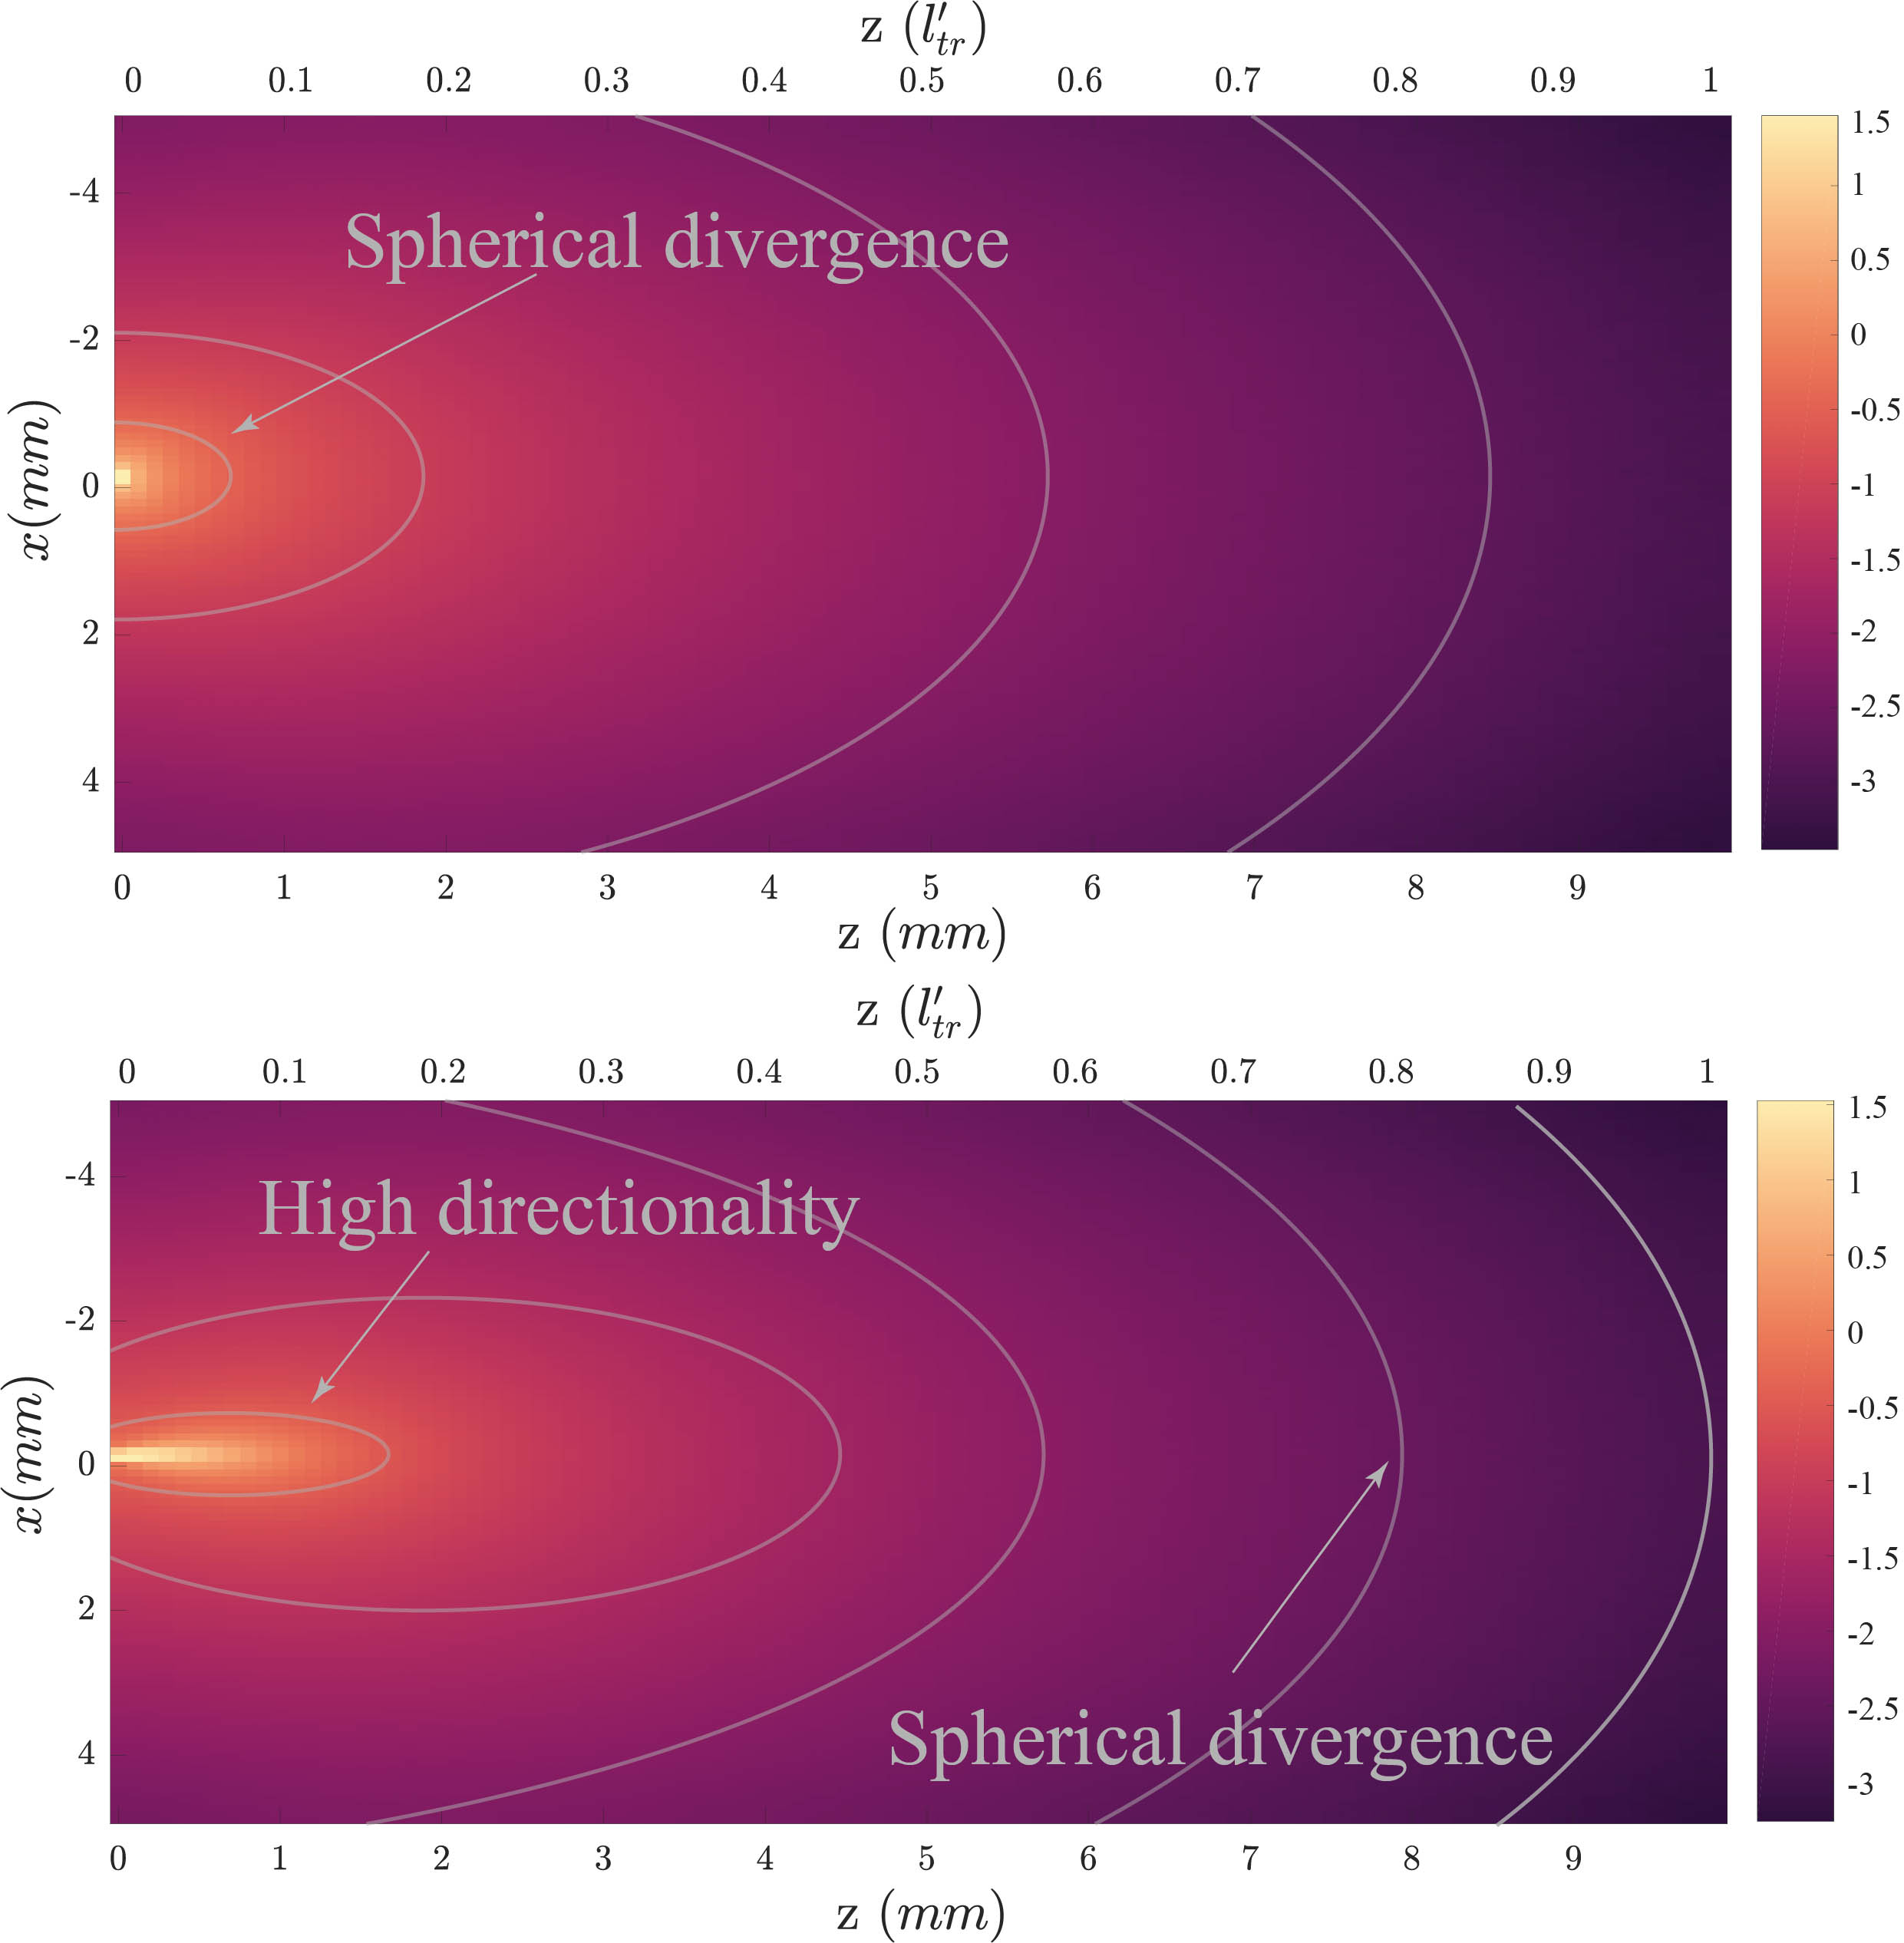
\includegraphics[width=1\textwidth]{near_infrared_theory/col_point_sources}
\caption[\gls{mc} simulations of a point source and a collimated beam]{\gls{mc} simulations using the MCX package~\cite{Fang2009} of an isotropic source (top) and a collimated gaussian beam (bottom) propagating in a medium with optical properties: $\mu_a=\SI[per-mode=reciprocal]{0.025}{\per\cm}$, $\mu'_s=\SI[per-mode=reciprocal]{1}{\per\cm}$.}
\label{fig:theory_col_point_src} 
\end{figure}

Although the simulations were performed using a relatively low scattering medium, it is easy to notice how directionality is nearly lost after just a few mm. In the case of a high scattering medium, this distance could have been lower than a millimeter. The quick loss of intensity also illustrates how difficult is to reach deep tissues. Even with low absorption, scattering would spread the light everywhere, inevitably reducing the intensity in the direction of propagation and leading to a uniform distribution of light in the distance.
(Fig.~\ref{fig:theory_propagation_3d})

Light diffusion also reduces the amount of information that light carries from the sample. To describe this effect, we need first to introduce the concept of spatial resolution. This key parameter in the evaluation of the performance of any imaging system quantifies its actual resolving power. Formally, it can be defined as the ability to separate images of two neighboring object points.

\begin{figure}[t!]
\centering
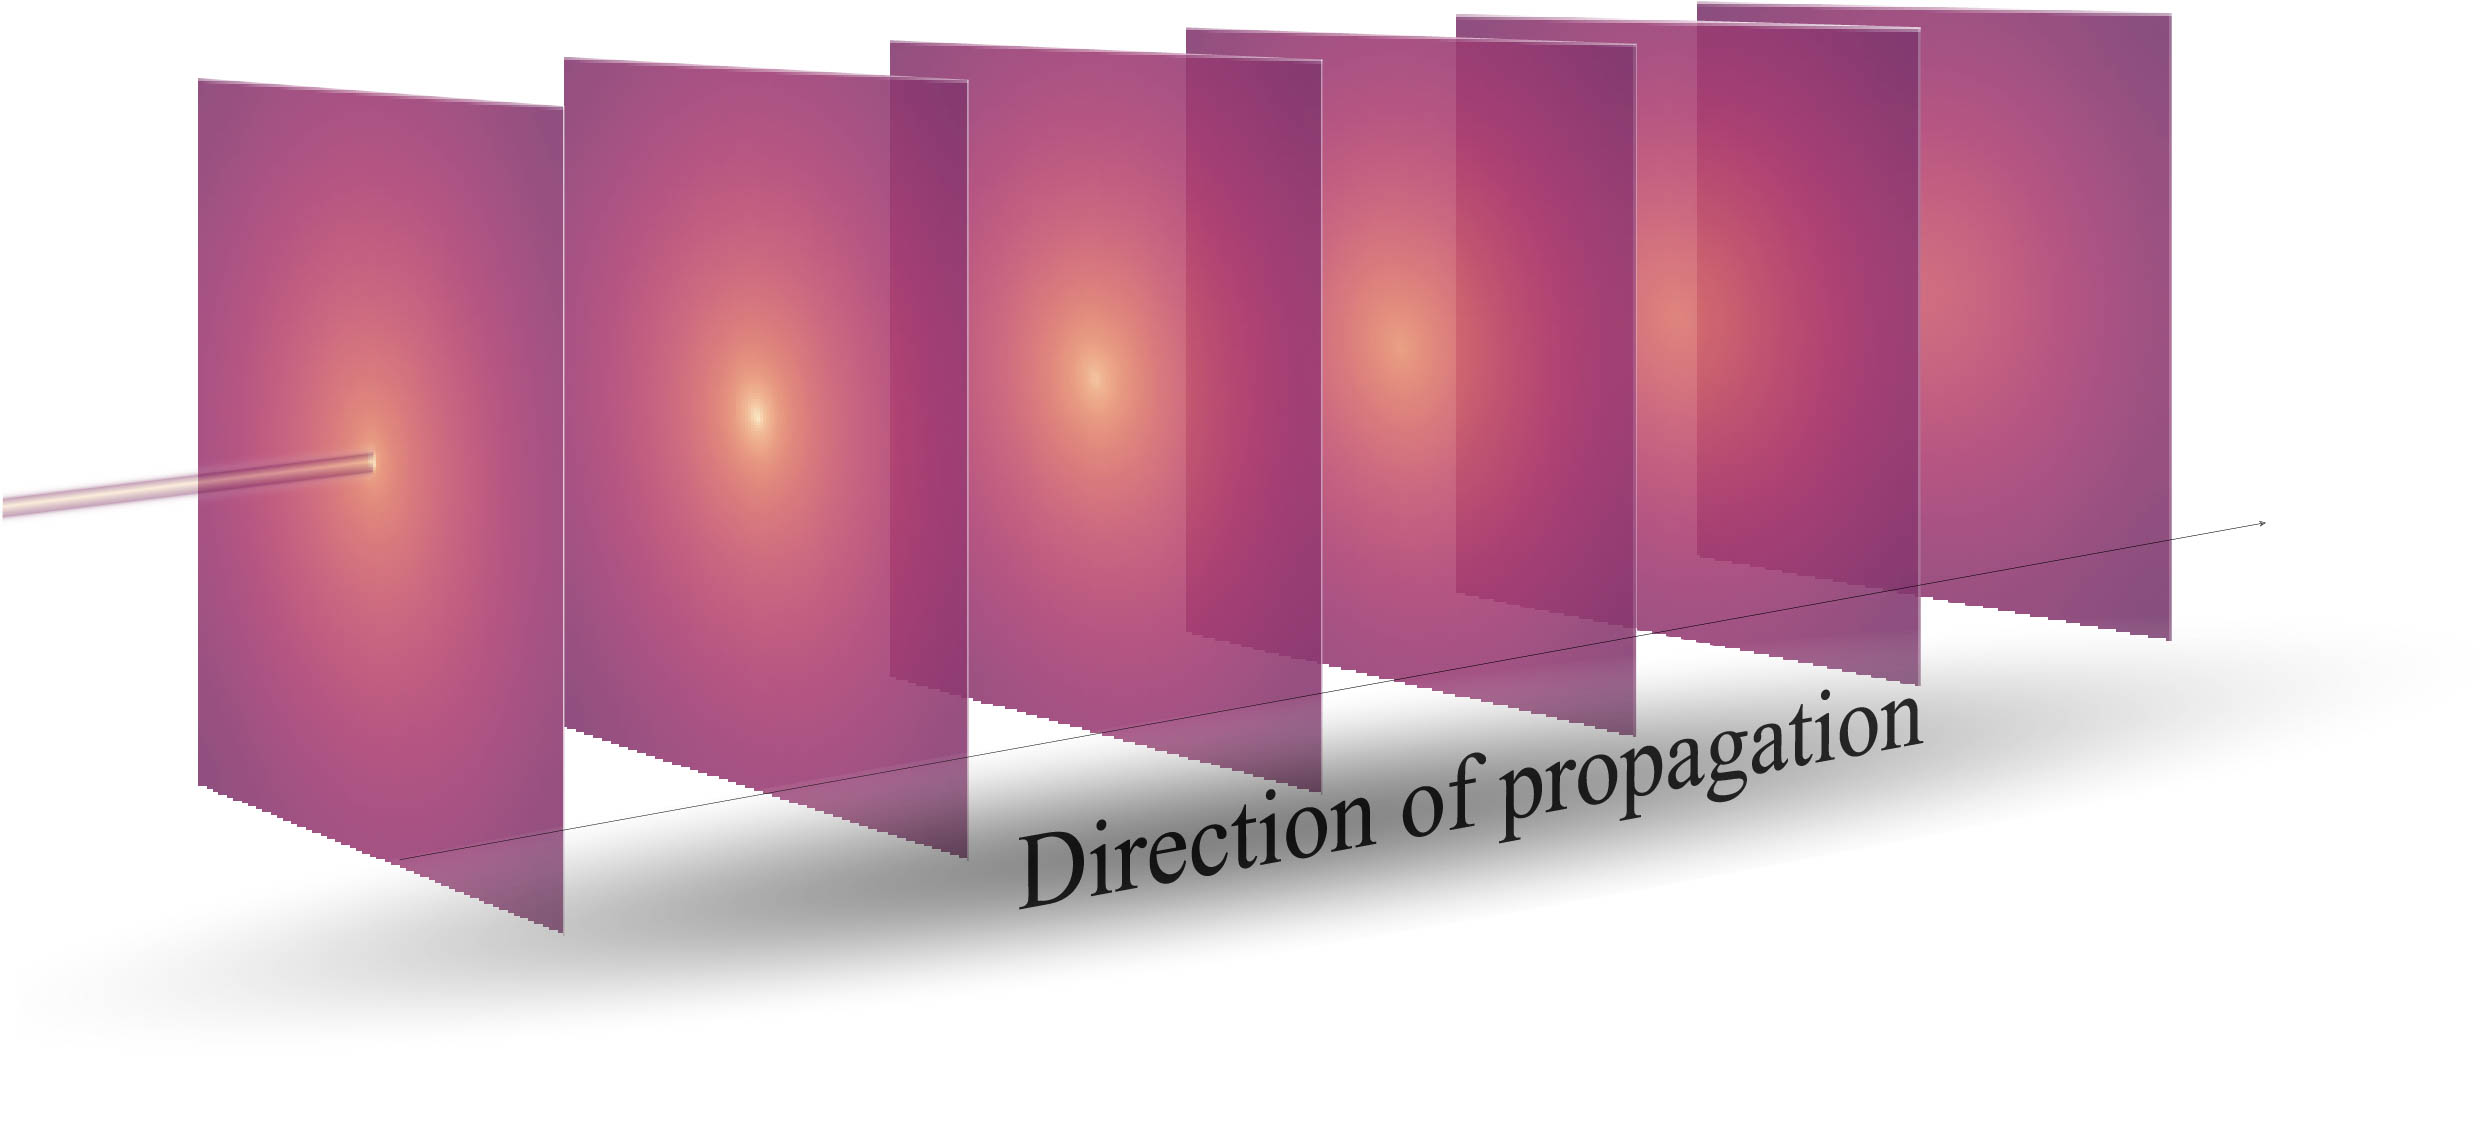
\includegraphics[width=1\textwidth]{near_infrared_theory/propagation_3d_size_arranged}
\caption[Propagation of a collimated source in an infinite medium]{Illustration of the propagation of a collimated source through an infinite medium with optical properties: $\mu_a=\SI[per-mode=reciprocal]{0.025}{\per\cm}$, $\mu'_s=\SI[per-mode=reciprocal]{1}{\per\cm}$. Images generated using simulations performed with Monte Carlo MCX package~\cite{Fang2009}.}
\label{fig:theory_propagation_3d} 
\end{figure}

In signal processing and engineering, a spatial frequency refers to the number of cycles of a sinusoidal per unit length. In the context to imaging, it can be said that high frequencies contain the information of fine details and sharp edges. The connection between spatial frequencies and resolution arises from the fact that the resolution limit of an image is the highest spatial frequency that can be resolved. Diffusion attenuates all frequencies, but this attenuation increases exponentially for higher spatial frequencies \cite{Ripoll1999}.

The response in the frequency domain in diffuse imaging can be predicted by the transfer function. This function describes how much each spatial frequency $K$ is attenuated due to the effect of propagation. The convolution between an incident field and the transfer function of the medium allows to estimate the intensity distribution at a certain plane $z$. The resolution limit at a certain distance can be obtained from the transfer function by measuring the full width half maximum (FWHM). This parameter is obtained by measuring the width of the lobe where the intensity falls to the half of its maximum value.
\begin{figure}[t!]
\centering
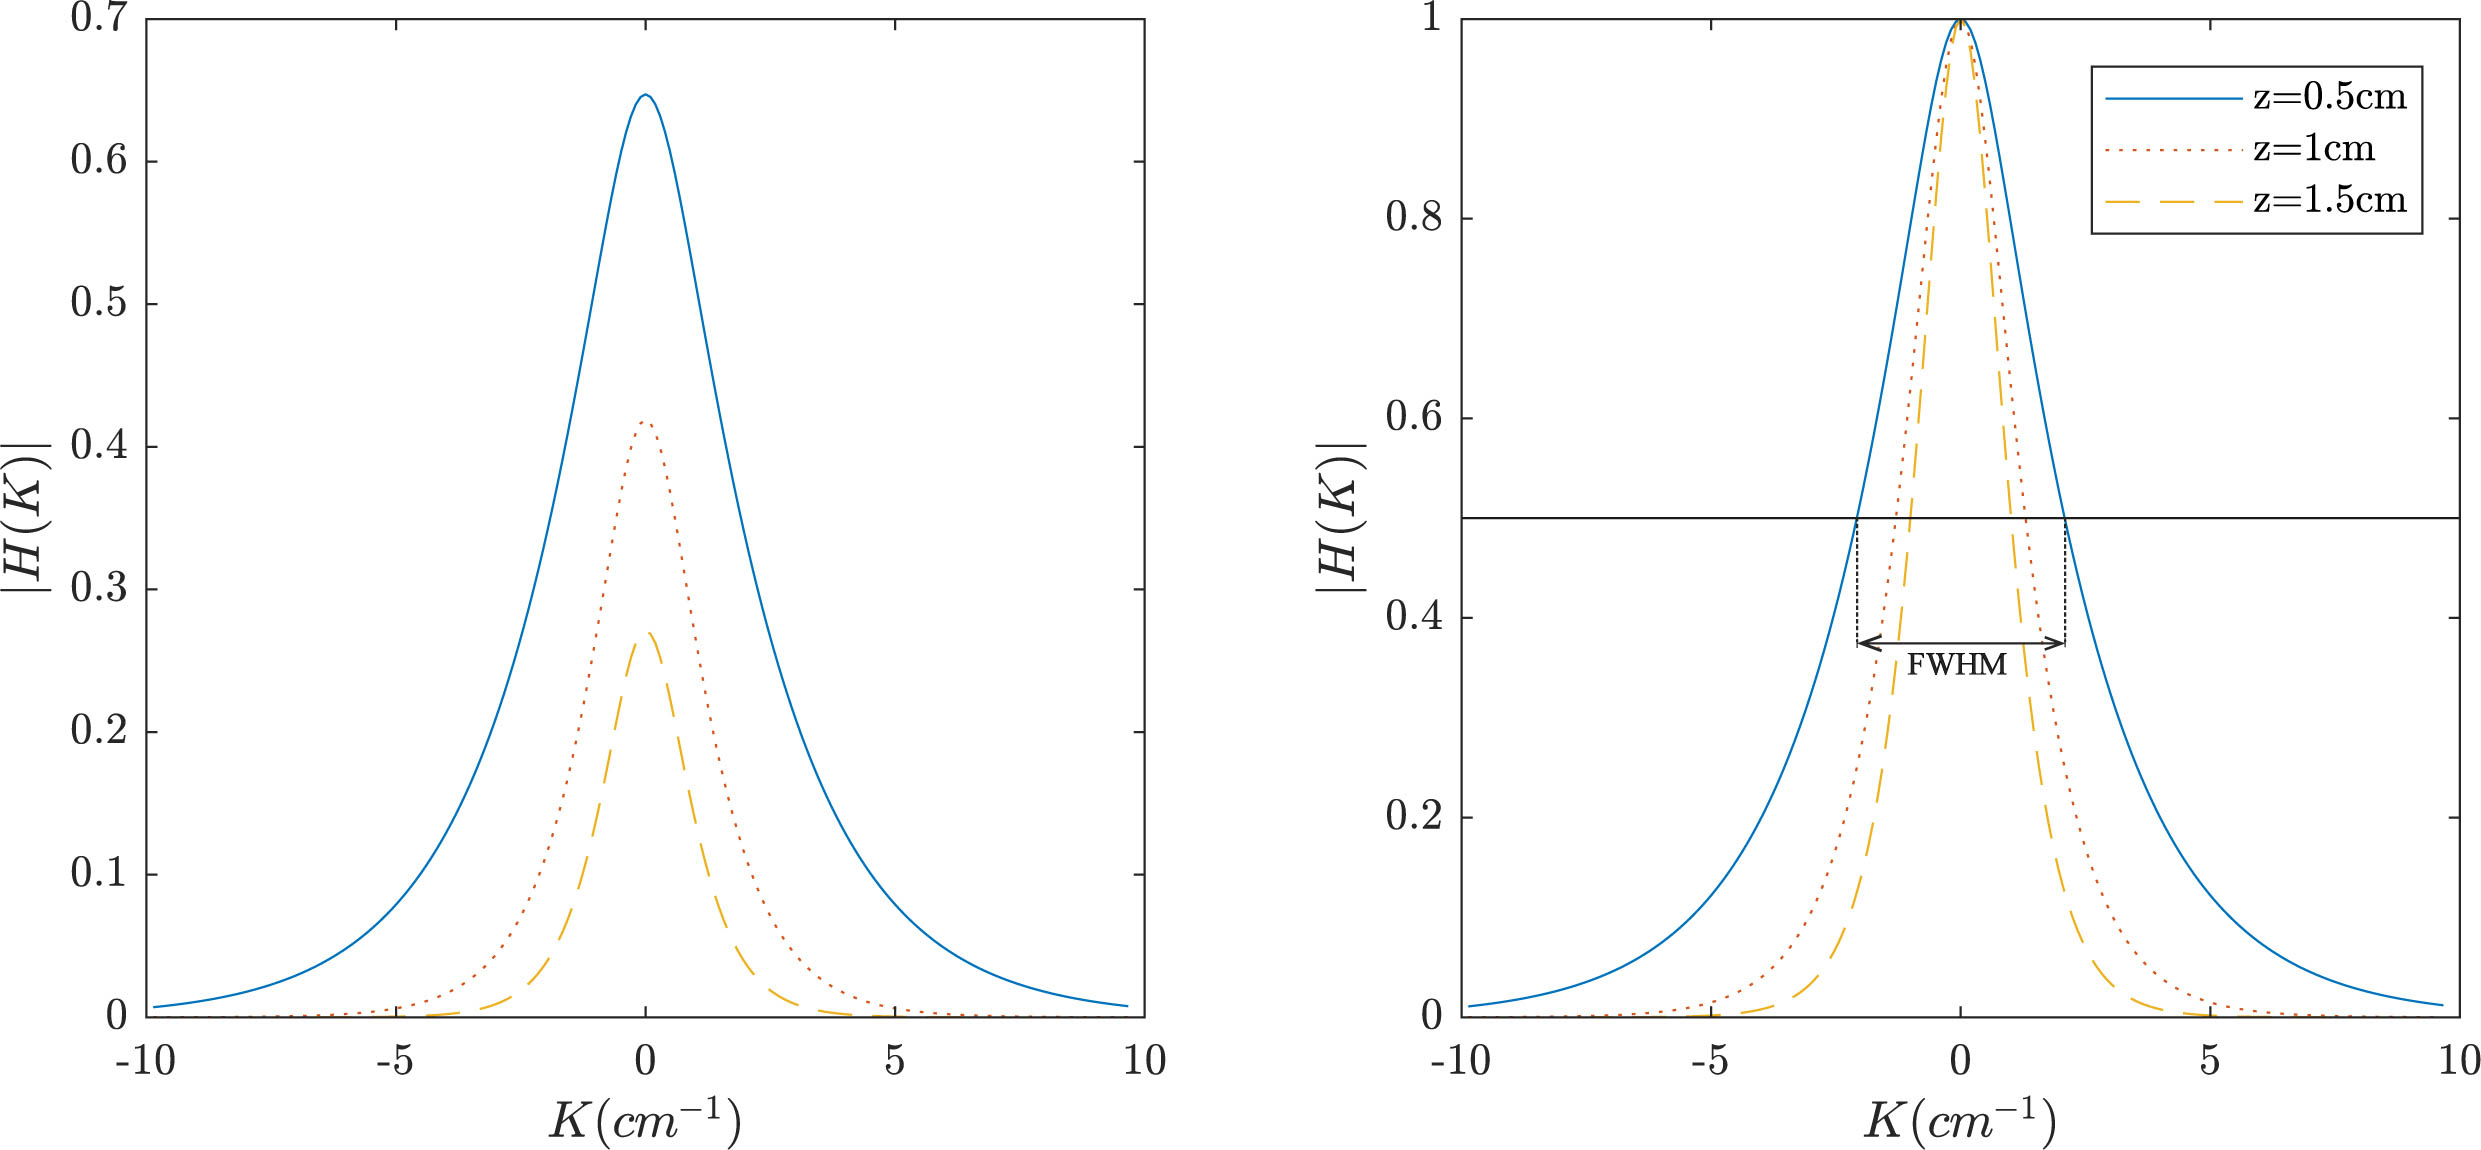
\includegraphics[width=1\textwidth]{near_infrared_theory/Hk}
\caption[Transfer function in a diffusive medium with optical properties {$\mu_a=\SI[per-mode=reciprocal]{0.025}{\per\cm}$}, {$\mu'_s=\SI[per-mode=reciprocal]{10}{\per\cm}$}]{Example values of the transfer function in a diffusive medium with optical properties $\mu_a=\SI[per-mode=reciprocal]{0.025}{\per\cm}$, $\mu'_s=\SI[per-mode=reciprocal]{10}{\per\cm}$. Right plot shows the values of the left plot normalized to the $K=0$ value. }
\label{fig:theory_transfer_function} 
\end{figure}

Figure~\ref{fig:theory_transfer_function} shows how the bandwidth decreases with distance while, at the same time, there is a global attenuation of the intensity for the entire frequency spectrum. This means that there is a quick loss of energy components in high frequency, thus acting as a low pass filter which narrows as we propagate deeper into the medium

\begin{figure}[b!]
\centering
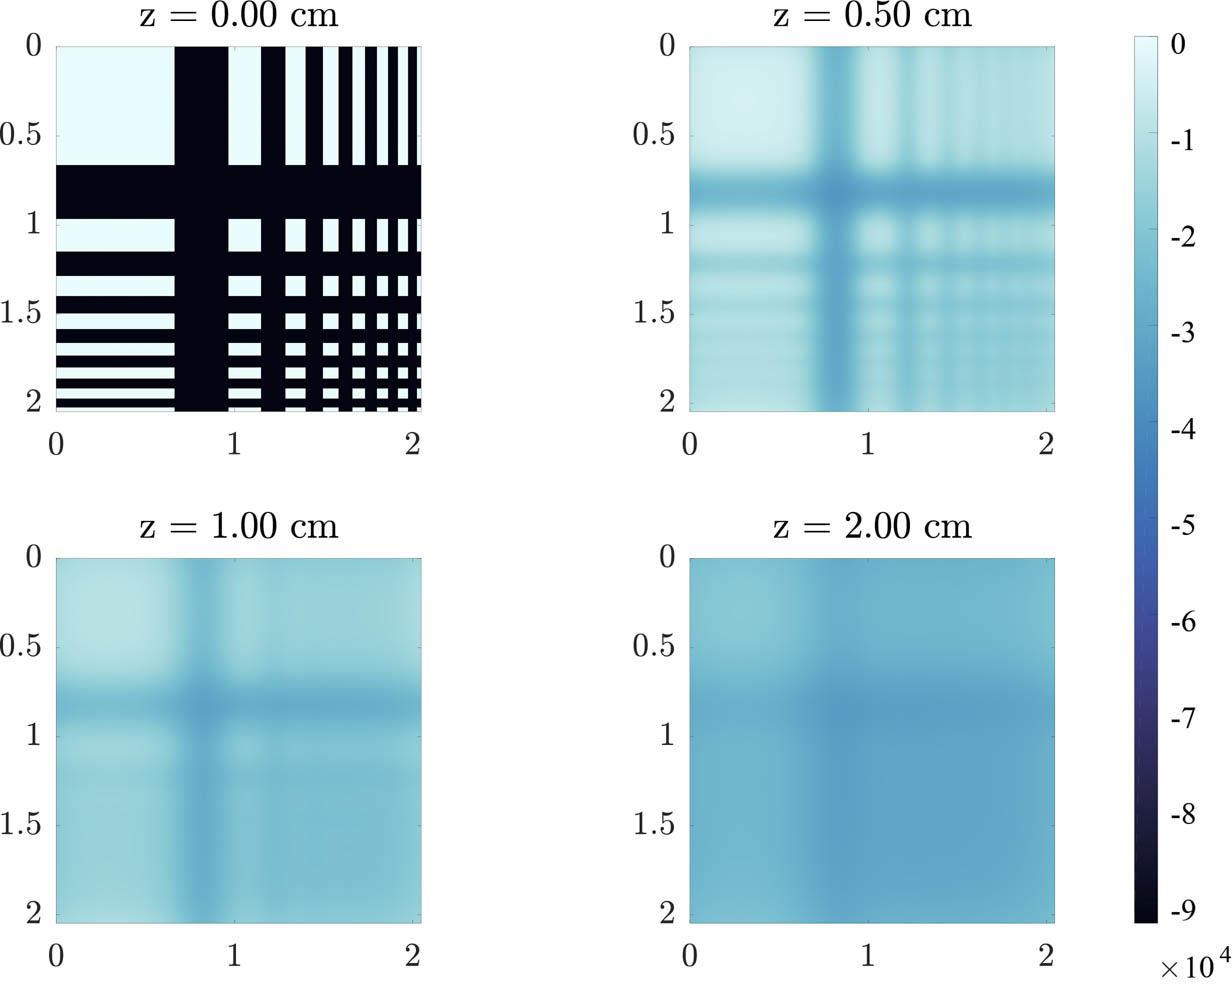
\includegraphics[width=0.85\textwidth]{near_infrared_theory/pattern_prop}
\caption[Simulation of the propagation of a pattern in diffusive media]{Simulation of the propagation of a pattern using the transfer function of a diffusive media with optical properties: $\mu_a=\SI[per-mode=reciprocal]{0.025}{\per\cm}$, $\mu'_s=\SI[per-mode=reciprocal]{10}{\per\cm}$. Intensities normalized with respect to $z = \SI{0}{\cm}$.}
\label{fig:theory_pattern prop}
\end{figure}

The main effect of low pass filtering an image is a loss of details, making it blurry. Figure \ref{fig:theory_pattern prop} gives an intuitive idea of these effects. After propagating a few millimeters, the smaller structures\textemdash high frequencies components\textemdash are nearly invisible. The loss of resolution affects also to the larger\textemdash low frequency components\textemdash which will become indistinguishable too after traveling slightly further in the medium. Also, the general intensity of the image decreases with propagation.

The consequences of light diffusion on quality are unavoidable, however, a reduced scattering and absorption medium can increase distance light may propagate without significant loss of resolution, reducing the spectral losses in the first millimeters and allowing a higher depth of penetration. This is the biggest advantage of using \gls{nir} light for imaging and the main reason for the high interest shown by the scientific community. Nowadays, the recent appearance of new \gls{nir} cameras sensitive to \gls{nir2}a and \gls{nir2}b windows, and the development of novel fluorescent probes in this range offer to researchers the possibility to take advantage of all the benefits that \gls{nir} light can bring into imaging.
